% Options for packages loaded elsewhere
\PassOptionsToPackage{unicode}{hyperref}
\PassOptionsToPackage{hyphens}{url}
%
\documentclass[
]{article}
\usepackage{lmodern}
\usepackage{amssymb,amsmath}
\usepackage{ifxetex,ifluatex}
\ifnum 0\ifxetex 1\fi\ifluatex 1\fi=0 % if pdftex
  \usepackage[T1]{fontenc}
  \usepackage[utf8]{inputenc}
  \usepackage{textcomp} % provide euro and other symbols
\else % if luatex or xetex
  \usepackage{unicode-math}
  \defaultfontfeatures{Scale=MatchLowercase}
  \defaultfontfeatures[\rmfamily]{Ligatures=TeX,Scale=1}
\fi
% Use upquote if available, for straight quotes in verbatim environments
\IfFileExists{upquote.sty}{\usepackage{upquote}}{}
\IfFileExists{microtype.sty}{% use microtype if available
  \usepackage[]{microtype}
  \UseMicrotypeSet[protrusion]{basicmath} % disable protrusion for tt fonts
}{}
\makeatletter
\@ifundefined{KOMAClassName}{% if non-KOMA class
  \IfFileExists{parskip.sty}{%
    \usepackage{parskip}
  }{% else
    \setlength{\parindent}{0pt}
    \setlength{\parskip}{6pt plus 2pt minus 1pt}}
}{% if KOMA class
  \KOMAoptions{parskip=half}}
\makeatother
\usepackage{xcolor}
\IfFileExists{xurl.sty}{\usepackage{xurl}}{} % add URL line breaks if available
\IfFileExists{bookmark.sty}{\usepackage{bookmark}}{\usepackage{hyperref}}
\hypersetup{
  pdftitle={C++ Neural Network in a Weekend},
  pdfauthor={Jeremy Ong},
  hidelinks,
  pdfcreator={LaTeX via pandoc}}
\urlstyle{same} % disable monospaced font for URLs
\usepackage{color}
\usepackage{fancyvrb}
\newcommand{\VerbBar}{|}
\newcommand{\VERB}{\Verb[commandchars=\\\{\}]}
\DefineVerbatimEnvironment{Highlighting}{Verbatim}{commandchars=\\\{\}}
% Add ',fontsize=\small' for more characters per line
\newenvironment{Shaded}{}{}
\newcommand{\AlertTok}[1]{\textcolor[rgb]{1.00,0.00,0.00}{\textbf{#1}}}
\newcommand{\AnnotationTok}[1]{\textcolor[rgb]{0.38,0.63,0.69}{\textbf{\textit{#1}}}}
\newcommand{\AttributeTok}[1]{\textcolor[rgb]{0.49,0.56,0.16}{#1}}
\newcommand{\BaseNTok}[1]{\textcolor[rgb]{0.25,0.63,0.44}{#1}}
\newcommand{\BuiltInTok}[1]{#1}
\newcommand{\CharTok}[1]{\textcolor[rgb]{0.25,0.44,0.63}{#1}}
\newcommand{\CommentTok}[1]{\textcolor[rgb]{0.38,0.63,0.69}{\textit{#1}}}
\newcommand{\CommentVarTok}[1]{\textcolor[rgb]{0.38,0.63,0.69}{\textbf{\textit{#1}}}}
\newcommand{\ConstantTok}[1]{\textcolor[rgb]{0.53,0.00,0.00}{#1}}
\newcommand{\ControlFlowTok}[1]{\textcolor[rgb]{0.00,0.44,0.13}{\textbf{#1}}}
\newcommand{\DataTypeTok}[1]{\textcolor[rgb]{0.56,0.13,0.00}{#1}}
\newcommand{\DecValTok}[1]{\textcolor[rgb]{0.25,0.63,0.44}{#1}}
\newcommand{\DocumentationTok}[1]{\textcolor[rgb]{0.73,0.13,0.13}{\textit{#1}}}
\newcommand{\ErrorTok}[1]{\textcolor[rgb]{1.00,0.00,0.00}{\textbf{#1}}}
\newcommand{\ExtensionTok}[1]{#1}
\newcommand{\FloatTok}[1]{\textcolor[rgb]{0.25,0.63,0.44}{#1}}
\newcommand{\FunctionTok}[1]{\textcolor[rgb]{0.02,0.16,0.49}{#1}}
\newcommand{\ImportTok}[1]{#1}
\newcommand{\InformationTok}[1]{\textcolor[rgb]{0.38,0.63,0.69}{\textbf{\textit{#1}}}}
\newcommand{\KeywordTok}[1]{\textcolor[rgb]{0.00,0.44,0.13}{\textbf{#1}}}
\newcommand{\NormalTok}[1]{#1}
\newcommand{\OperatorTok}[1]{\textcolor[rgb]{0.40,0.40,0.40}{#1}}
\newcommand{\OtherTok}[1]{\textcolor[rgb]{0.00,0.44,0.13}{#1}}
\newcommand{\PreprocessorTok}[1]{\textcolor[rgb]{0.74,0.48,0.00}{#1}}
\newcommand{\RegionMarkerTok}[1]{#1}
\newcommand{\SpecialCharTok}[1]{\textcolor[rgb]{0.25,0.44,0.63}{#1}}
\newcommand{\SpecialStringTok}[1]{\textcolor[rgb]{0.73,0.40,0.53}{#1}}
\newcommand{\StringTok}[1]{\textcolor[rgb]{0.25,0.44,0.63}{#1}}
\newcommand{\VariableTok}[1]{\textcolor[rgb]{0.10,0.09,0.49}{#1}}
\newcommand{\VerbatimStringTok}[1]{\textcolor[rgb]{0.25,0.44,0.63}{#1}}
\newcommand{\WarningTok}[1]{\textcolor[rgb]{0.38,0.63,0.69}{\textbf{\textit{#1}}}}
\usepackage{longtable,booktabs}
% Correct order of tables after \paragraph or \subparagraph
\usepackage{etoolbox}
\makeatletter
\patchcmd\longtable{\par}{\if@noskipsec\mbox{}\fi\par}{}{}
\makeatother
% Allow footnotes in longtable head/foot
\IfFileExists{footnotehyper.sty}{\usepackage{footnotehyper}}{\usepackage{footnote}}
\makesavenoteenv{longtable}
\usepackage{graphicx}
\makeatletter
\def\maxwidth{\ifdim\Gin@nat@width>\linewidth\linewidth\else\Gin@nat@width\fi}
\def\maxheight{\ifdim\Gin@nat@height>\textheight\textheight\else\Gin@nat@height\fi}
\makeatother
% Scale images if necessary, so that they will not overflow the page
% margins by default, and it is still possible to overwrite the defaults
% using explicit options in \includegraphics[width, height, ...]{}
\setkeys{Gin}{width=\maxwidth,height=\maxheight,keepaspectratio}
% Set default figure placement to htbp
\makeatletter
\def\fps@figure{htbp}
\makeatother
\setlength{\emergencystretch}{3em} % prevent overfull lines
\providecommand{\tightlist}{%
  \setlength{\itemsep}{0pt}\setlength{\parskip}{0pt}}
\setcounter{secnumdepth}{-\maxdimen} % remove section numbering
\usepackage{amsmath}
\usepackage{tikz}
\usepackage{mathtools}
\usepackage{amsthm}
\usepackage{amssymb}
\usepackage{bm}
\usetikzlibrary{positioning}
\usetikzlibrary{arrows}
\usetikzlibrary{shapes}
\usetikzlibrary{calc}
\ifluatex
  \usepackage{selnolig}  % disable illegal ligatures
\fi

\title{C++ Neural Network in a Weekend}
\author{Jeremy Ong}
\date{}

\begin{document}
\maketitle

\hypertarget{introduction}{%
\subsection{Introduction}\label{introduction}}

Would you like to write a neural network from start to finish? Are you
perhaps shaky on some of the fundamental concepts and derivations, such
as categorical cross-entropy loss or backpropagation? Alternatively,
would you like an introduction to machine learning without relying on
``magical'' frameworks that seem to perform AI miracles with only a few
lines of code (and just as little intuition)? If so, this article was
written for you.

Deep learning as a technology and discipline has been booming. Nearly
every facet of deep learning is teeming with progress and healthy
competition to achieve state of the art performance and efficiency. It's
no surprise that resources tend to emphasize the ``latest and greatest''
in feats such as object recognition, natural language parsing, ``deep
fakes'', and more. In contrast, fewer resources expand as much on the
practical \emph{engineering} aspects of deep learning. That is, how
should a deep learning framework be structured? How do you go about
rolling your own infrastructure instead of relying on Keras, Pytorch,
Tensorflow, or any of the other dominant frameworks? Whether you wish to
write your own for learning purposes, or if you need to deploy a neural
network on a constrained (i.e.~embedded) device, there is plenty to be
gained from authoring a neural network from scratch.

The neural network outlined here is hosted on
\href{https://github.com/jeremyong/cpp_nn_in_a_weekend}{github} and has
enough abstractions to vaguely resemble a production network, without
being overly engineered as to be indigestible in a sitting or two. The
training and test data provided is the venerable
\href{http://yann.lecun.com/exdb/mnist/}{MNIST} dataset of handwritten
digits. While more exotic (and original) datasets exist, MNIST is chosen
here because its sheer ubiquity guarantees you can find corresponding
literature to help drive further experimentation, or troubleshoot when
things go wrong.

\hypertarget{background}{%
\subsection{Background}\label{background}}

This section serves as a moderately high-level description of the major
mathematical underpinnings of neural networks and may be safely skipped
by those who prefer to jump straight to the code.

Suppose we have a task we would like a machine learning model to
complete (e.g.~recognizing handwritten digits). At a high level, we need
to perform the following tasks:

\begin{enumerate}
\def\labelenumi{\arabic{enumi}.}
\tightlist
\item
  First, we must conceptualize the task as a ``function'' such that the
  inputs and outputs of the task can be described in a concrete
  mathematical sense (amenable for programmability).
\item
  Second, we need a way to quantify the degree to which our model is
  performing poorly against a known set of correct answers. This is
  typically denoted as the \emph{loss} or \emph{objective} function of
  the model.
\item
  Third, we need an \emph{optimization strategy} which will describe how
  to adjust the model after feedback is provided regarding the model's
  performance as per the loss function described above.
\item
  Fourth, we need a \emph{regularization strategy} to address
  inadvertently tuning the model with a high degree of specificity to
  our training data, at the cost of generalized performance when
  handling inputs not yet encountered.
\item
  Fifth, we need an \emph{architecture} for our model, including how
  inputs are transformed into outputs and an enumaration of all the
  adjustable parameters the model supports.
\item
  Finally, we need a robust \emph{implementation} that executes the
  above within memory and execution budgets, accounting for
  floating-point stability, reproducibility, and a number of other
  engineering-related matters.
\end{enumerate}

\emph{Deep learning} is distinct from other machine learning models in
that the architecture is heavily over-parameterized and based on simpler
\emph{building blocks} as opposed to bespoke components. The building
blocks used are neurons, or particular arrangements of neurons,
typically organized as layers. Over the course of training a deep
learning model, it is expected that \emph{features} of the inputs are
learned and manifested as various parameter values in these neurons.
This is in contrast to traditional machine learning, where features are
not learned, but implemented directly.

\hypertarget{categorical-cross-entropy-loss}{%
\subsubsection{Categorical Cross-Entropy
Loss}\label{categorical-cross-entropy-loss}}

More concretely, the task at hand is to train a model to recognize a 28
by 28 pixel handwritten greyscale digit. For simplicity, our model will
interpret the data as a flattened 784-dimensional vector. Instead of
describing the architecture of the model first, we'll start with
understanding what the model should output and how to assess the model's
performance. The output of our model will be a 10-dimensional vector,
representing the probability distribution of the supplied input. That
is, each element of the output vector indicates the model's estimation
of the probability that the digit's value matches the corresponding
element index. For example, if the model outputs:

\[M(\mathbf{I}) = \left[0, 0, 0.5, 0.5, 0, 0, 0, 0, 0, 0\right]\]

for some input image \(\mathbf{I}\), we interpret this to mean that the
model believes there is an equal chance of the examined digit to be a 2
or a 3.

Next, we should consider how to quantify the model's loss. Suppose, for
example, that the image \(\mathbf{I}\) actually corresponded to the
digit ``7'' (our model made a horrible prediction!), how might we
penalize the model? In this case, we know that the \emph{actual}
probability distribution is the following:

\[\left[0, 0, 0, 0, 0, 0, 0, 1, 0, 0\right]\]

This is known as a ``one-hot'' encoded vector, but it may be helpful to
think of it as a probability distribution given a set of events that are
mutually exclusive (a digit cannot be both a ``7'' \emph{and} a ``3''
for instance).

Fortunately, information theory provides us some guidance on defining an
easy-to-compute loss function which quantifies the dissimilarities
between two probability distributions. If the probability of of an event
\(E\) is given as \(P(E)\), then the \emph{entropy} of this event is
given as \(-\log P(E)\). The negation ensures that this is a positive
quantity, and by inspection, the entropy increases as an event becomes
less likely. Conversely, in the limit as \(P(E)\) approaches \(1\), the
entropy shrinks to \(0\). While several interpretations of entropy are
possible, the pertinent interpretation here is that entropy is a
\emph{measure of the information conveyed when a particular event
occurs}. That the ``sun rose this morning'' is a fairly mundane
observation but being told ``the sun exploded'' is sure to pique your
attention. Because we are reasonably certain that the sun rises each
morning (with near 100\% confidence), that ``the sun rises'' is an event
that conveys little additional information when it occurs.

Let's consider next entropy in the context of a probability
distribution. Given a discrete random variable \(X\) which can take on
values \(x_0, \dots, x_{n-1}\) with probabilities
\(p(x_0), \dots, p(x_{n-1})\), the entropy of the random variable \(X\)
is defined as:

\[H(X) = -\sum_{x \in X} p(x) \log p(x)\]

For example, suppose \(W\) is a binary random variable that represents
today's weather which can either be ``sunny'' or ``rainy'' (a binary
random variable). The entropy \(H(W)\) can be given as:

\[H(W) = -S\log S - (1 - S) \log (1 - S)\]

where \(S\) is the probability of a sunny day, and hence \(1 - S\) is
the probability of a rainy day. As a binary random variable, the
summation over weighted entropies expands to only two terms. What does
this quantity mean? If we were to describe it in words, each term of the
sum in the entropy calculation corresponds to the information of a
particular event, weighted by the probability of the event. Thus, the
entropy of the distribution is literally the \emph{expected amount of
information contained in an event} for a given distribution. If we plot
\(-S\log S - (1 - S) \log(1 - S)\) as a function of \(S\), we will see
something like this:

\begin{figure}
\centering
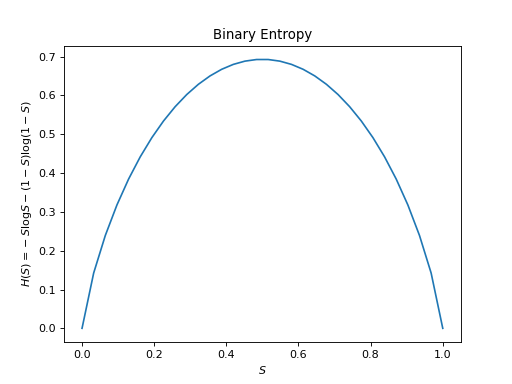
\includegraphics{plots/6094492350593652429.png}
\caption{}
\end{figure}

As a minor note, while \(\log 0\) is an undefined quantity, information
theorists accept that \(\lim_{p\rightarrow 0} p\log p = 0\) by
convention. Intuitively, the expected entropy should be unaffected by
the set of impossible events.

As you might expect, when the distribution is 50-50, the uncertainty of
a binary is maximal, and by extension the amount of information
contained in each event is maximized too. Put another way, if you lived
in an area where it was always sunny, you wouldn't \emph{learn anything}
if someone told you it was sunny today. However, in a tropical region
characterized by capricious weather, information conveyed about the
weather is far more meaningful.

In the previous example, we weighted the event entropies according to
the event's probability distribution. What would happen if, instead, we
used weights corresponding to a \emph{different} probability
distribution? This is known as the \emph{cross entropy}:

\[H(p, q) = -\sum_{x \in X} p(x)\log q(x)\]

To get some intuition about this, first, we note that if
\(p(x) = q(x), \forall x\in X\), the cross entropy trivially matches the
self-entropy. Let's go back to our binary entropy example and visualize
what it looks like if we chose a completely \emph{incorrect}
distribution. Specifically, suppose we computed the cross entropy where
if the probability of a sunny day is \(S\), we weight the entropy with
\(1 - S\) instead of \(S\) as in the self-entropy formula.

\begin{figure}
\centering
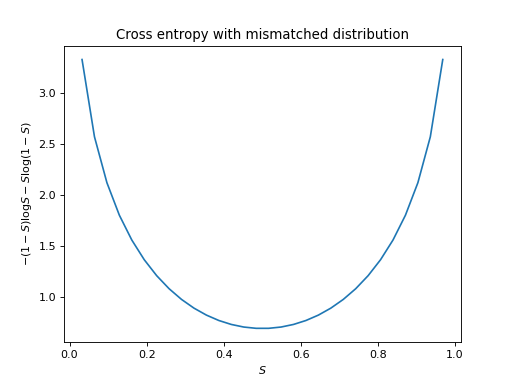
\includegraphics{plots/-6767785830879840565.png}
\caption{}
\end{figure}

If you compare the values with the previous figure, you'll see that the
cross entropy diverges from the self-entropy everywhere except \(0.5\),
where \(S = 1 - S\). The difference between the cross entropy
\(H(p, q)\) and entropy \(H(p)\) provides then, a \emph{measure of
error} between the presumed distribution \(q\) and the true distribution
\(p\). This difference is also known as the
\href{https://en.wikipedia.org/wiki/Kullback\%E2\%80\%93Leibler_divergence}{Kullback-Leibler
divergence} or KL divergence for short.

Given that the entropy of a given probability distribution \(p\) is
constant, then \(H(p)\) must be constant as well. This is why in
practice, we will generally seek to minimize the cross entropy between
\(p\) and a predicted distribution \(q\), which by extension will
minimize the Kullback-Leibler divergence as well.

Now, we have the tools to know if our model is succeeding or not! Given
an estimation of a sample's label as before:

\[M(\mathbf{I}) = \left[0, 0, 0.5, 0.5, 0, 0, 0, 0, 0, 0\right]\]

we will treat our model's output as a predicted probability distribution
of the sample digit's classification from 0 to 9. Then, we compute the
cross entropy between this predction and the true distribution, which
will be in the form of a one-hot vector. Supposing the actual digit is 3
in this particular case (\(P(7) = 1\)):

\[ \sum_{x\in \{0,\dots, 9\}} -P(x) \log Q(x) = -P(3) \log(Q(3)) = \log(0.5) \approx 0.301 \]

Let's make a few observations before continuing. First, for a one-hot
vector, the entropy is 0 (can you see why?). Second, by pretending the
correct digit above is \(3\) and not, say, \(7\), we conveniently
avoided \(\log 0\) showing up in the final expression. A common method
to avoid this is to add a small \(\epsilon\) to the log argument to
avoid this singularity, but we'll discuss this in more detail later.

\hypertarget{creating-our-approximation-function-with-a-neural-network}{%
\subsubsection{Creating our Approximation Function with a Neural
Network}\label{creating-our-approximation-function-with-a-neural-network}}

Now that we know how to evaluate our model, we'll need to decide how to
go about making predictions in the form of a probability distribution.
Our model will need to take as inputs, 28x28 images (which as mentioned
before, will be flattened to 784x1 vectors for simplicity). Let's
enumerate the properties our model will need:

\begin{enumerate}
\def\labelenumi{\arabic{enumi}.}
\tightlist
\item
  Parameterization - our model will need parameters we can adjust to
  ``fit'' the model to the data
\item
  Nonlinearity - it is assuredly not the case that the probability
  distribution can be modeled with a set of linear equations
\item
  Differentiability - the gradient of our model's output with respect to
  any given parameter indicates the \emph{impact} of that parameter on
  the final result
\end{enumerate}

There are an infinite number of functions that fit this criteria, but
here, we'll use a simple feedforward network with a single hidden layer.

\begin{center}
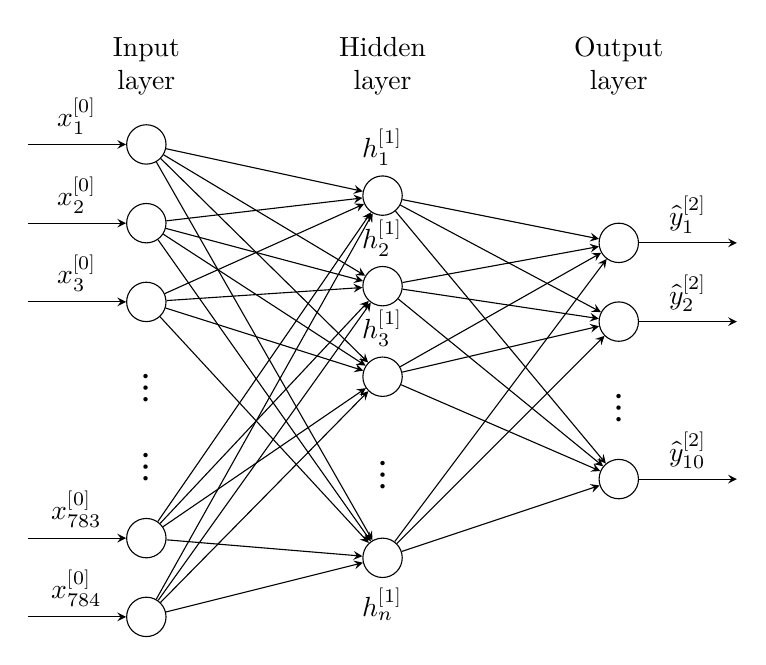
\begin{tikzpicture}[x=1.5cm, y=1cm, >=stealth]

\tikzset{%
    every neuron/.style = {
        circle,
        draw,
        minimum size=0.5cm
    },
    neuron missing/.style = {
        draw=none,
        scale=1.5,
        text height=0.3333cm,
        execute at begin node=\color{black}$\vdots$
    }
}


\foreach \m/\l [count=\y] in {1,2,3,missing,missing,783,784}
  \node [every neuron/.try, neuron \m/.try] (input-\m) at (0,2.5-\y) {};

\foreach \m [count=\y] in {1,2,3,missing,4}
  \node [every neuron/.try, neuron \m/.try ] (hidden-\m) at (2,2-\y*1.15) {};

\foreach \m [count=\y] in {1,2,missing,10}
  \node [every neuron/.try, neuron \m/.try ] (output-\m) at (4,1.25-\y) {};

\foreach \l in {1,2,3,783,784}
  \draw [<-] (input-\l) -- ++(-1,0)
    node [above, midway] {$x_{\l}^{[0]}$};

\foreach \l [count=\i] in {1,2,3}
  \node [above] at (hidden-\i.north) {$h_\l^{[1]}$};

\node [below] at (hidden-4.south) {$h_n^{[1]}$};

\foreach \l in {1,2,10}
  \draw [->] (output-\l) -- ++(1,0)
    node [above, midway] {$\hat{y}_{\l}^{[2]}$};

\foreach \i in {1,2,3,783,784}
{
  \draw [->] (input-\i) -- (hidden-4);
  \foreach \j in {1,...,3}
    \draw [->] (input-\i) -- (hidden-\j);
}

\foreach \i in {1,2,3,4}
{
  \draw [->] (hidden-\i) -- (output-10);
  \foreach \j in {1,...,2}
    \draw [->] (hidden-\i) -- (output-\j);
}

\foreach \l [count=\x from 0] in {Input, Hidden, Output}
  \node [align=center, above] at (\x*2,2) {\l \\ layer};

\end{tikzpicture}
\end{center}

A few quick notes regarding notation: a superscript of the form \([i]\)
is used to denote the \(i\)th layer. A subscript is used to denote a
particular element within a layer or vector. The vector \(\mathbf{x}\)
is usually reserved for training samples, and the vector \(\mathbf{y}\)
is typically reserved for sample labels (i.e.~the desired ``answer'' for
a given sample). The vector \(\hat{\mathbf{y}}\) is used to denote a
model's predicted labels for a given input.

On the far left, we have the input layer with \(784\) nodes
corresponding to each of the 28 by 28 pixels in an individual sample.
Each \(x_i^{(0)}\) is a floating point value between 0 and 1 inclusive.
Because the data is encoded with 8 bits of precision, there are 256
possible values for each input. Each of the 784 input values fan out to
each of the nodes in the hidden layer without modification.

In the center hidden layer, we have a variable number of nodes that each
receive all 784 inputs, perform some processing, and fan out the result
to the output nodes on the far right. That is, each node in the hidden
layer transforms a \(\mathbb{R}^{784}\) vector into a scalar output, so
as a whole, the \(n\) nodes collectively need to map
\(\mathbb{R}^\rightarrow \mathbb{R}^n\). The simplest way to do this is
with an \(n\times 784\) matrix (treating inputs as column vectors).
Modeling the hidden layer this way, each of the \(n\) nodes in the
hidden layer is associated with a single row in our
\(\mathbb{R}^{n\times 784}\) matrix. Each entry of this matrix is
referred to as a \emph{weight}.

We still have two issues we need to address however. First, a matrix
provides a linear mapping between two spaces, and linear maps take \(0\)
to \(0\) (you can visualize such maps as planes through the origin).
Thus, such fully-connected layers typically add a \emph{bias} to each
output node to turn the map into an affine map. This enables the model
to respond zeroes in the input. Thus, the hidden layer as a whole has
now both a weight matrix, and also a bias vector. A linear mapping with
a constant bias is commonly referred to as an \emph{affine map}.

The second issue is that our hidden layer's now-affine mapping still
scales linearly with the input, and one of our requirements for our
approximation function was nonlinearity (a strict prerequisite for
universality). Thus, we perform one final non-linear operation the
result of the affine map. This is known as the \emph{activation
function}, and an infinite number of choices present itself here. In
practice, the \emph{rectifier function}, defined below, is a perennial
choice.

\[f(x) = \max(0, x)\]

\begin{figure}
\centering
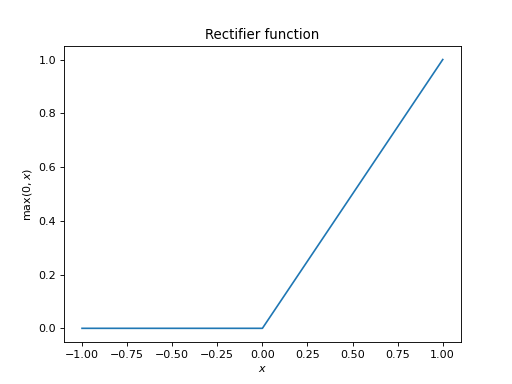
\includegraphics{plots/-1637788021081228918.png}
\caption{}
\end{figure}

The rectifier is popular for having a number of desirable properties.

\begin{enumerate}
\def\labelenumi{\arabic{enumi}.}
\tightlist
\item
  Easy to compute
\item
  Easy to differentiate (except at 0, which has not been found to be a
  problem in practice)
\item
  Sparse activation, which aids in addressing model overfitting and
  ``unlearning'' useful weights
\end{enumerate}

As our hidden layer units will use this rectifier just before emitting
its final output to the next layer, our hidden units may be called
\emph{rectified linear units} or ReLUs for short.

Summarizing our hidden layer, the output of each unit in the layer can
be written as:

\[a_i^{[1]} = \max(0, W_{i}^{[1]} \cdot \mathbf{x}^{[0]} + b_i^{[1]})\]

It's common to refer to the final activated output of a neural network
layer as the vector \(\mathbf{a}\), and the result of the internal
affine map \(\mathbf{z}\). Using this notation and considering the
output of the hidden layer as a whole as a vector quantity, we can
write:

\[
\begin{aligned}
\mathbf{z}^{[1]} &= \mathbf{W}^{[1]}\mathbf{x}^{[0]} + \mathbf{b}^{[1]} \\
\mathbf{a}^{[1]} &= \max(\mathbf{0}, \mathbf{z}^{[1]}) \\
\mathbf{a}^{[1]}, \mathbf{b}^{[1]} &\in \mathbb{R}^n \\
\mathbf{W}^{[1]} &\in \mathbb{R}^{n\times 784} \\
\mathbf{x}^{[0]} &\in \mathbb{R}^{784}
\end{aligned}
\]

The last layer to consider is the output layer. As with the hidden
layer, we need a dimensionality transform, in this case, taking vectors
in \(\mathbb{R}^n\) and mapping them to vectors in \(\mathbb{R}^{10}\)
(corresponding to the 10 possible digits in the target output). As
before, we will use an affine map with the appropriately sized weight
matrix and bias vector. Here, however, the rectifier isn't suitable as
an activation function because we want to emit a probability
distribution. To be a valid probability distribution, each output of the
hidden layer must be in the range \([0, 1]\), and the sum of all outputs
must equal \(1\). The most common activation function used to achieve
this is the \emph{softmax function}:

\[\mathrm{softmax}(\mathbf{z})_i = \frac{\exp(z_i)}{\sum_j \exp(z_j)}\]

Given a vector input \(z\), each component of the softmax output (as a
vector quantity) is given as per the expression above. The exponential
functions conveniently map negative numbers to positive numbers, and the
denominator ensures that all outputs will be between 0 and 1, and sum to
1 as desired. There are other reasons why an exponential function is
used here, stemming from our choice of a loss function (based on the
underpinning notion of maximum-likelihood estimation), but we won't get
into that in too much detail here (consult the further reading section
at the end to learn more). Suffice it to say that an additional benefit
of the exponential function is its clean interaction with the logarithm
used in our choice of loss function, especially when we will need to
compute gradients in the next section.

Summarizing our neural network architecture, with two weight matrices
and two bias vectors, we can construct two affine maps which map vectors
in \(\mathbb{R}^{784}\) to \(\mathbb{R}^n\) to \(\mathbb{R}^{10}\).
Prior to forwarding the results of one affine map as the input of the
next, we employ an activation function to add non-linearity to the
model. First, we use a linear rectifier and second, we use a softmax
function, ensuring that we end up with a nice discrete probability
distribution with 10 possible events corresponding to the 10 digits.

Our network is small enough that we can actually write out the entire
process as a single function using the notation we've built so far:

\[f(\mathbf{x}^{[0]}) = \mathbf{y}^{[2]} = \mathrm{softmax}\left(\mathbf{W}^{[2]}\left(\max\left(\mathbf{0}, \mathbf{W}^{[1]}\mathbf{x}^{[0]} + \mathbf{b}^{[1]}\right) \right) + \mathbf{b}^{[1]} \right)\]

\hypertarget{optimizing-our-network}{%
\subsubsection{Optimizing our network}\label{optimizing-our-network}}

We now have a model given above which can turn our 784 dimensional
inputs into a 10-element probability distribution, \emph{and} we have a
way to evaluate how accuracy of each prediction. Next, we need a
reliable way to improve the model based on the feedback provided by our
loss function. This is known as function \emph{optimization}, and most
methods of model optimization are based on the principle of
\emph{gradient descent}.

The idea is quite simple. Given a function with a set of parameters
which we'll denote \(\bm{\theta}\), the partial derivative of that
function with respect to a given parameter \(\theta_i \in \bm{\theta}\)
tells us the overall \emph{impact} of \(\theta_i\) on the final result.
In our model, we have many parameters; each weight and bias constitutes
an individually tunable parameter. Thus, our strategy should be, given a
set of input samples, compute the loss our model produces for each
sample. Then, compute the partial derivatives of that loss with respect
to \emph{every parameter} in our model. Finally, adjust each parameter
in proportion to its impact on the final loss. Mathematically, this
process is described below (note that the superscript \((i)\) is used to
denote the \(i\)-th sample):

\[
\begin{aligned}
\mathrm{Total~Loss} &= \sum_i J(\mathbf{x}^{(i)}; \bm\theta) \\
\mathrm{Compute}~ &\sum_i \frac{\partial J(\mathbf{x}^{(i)})}{\partial \theta_j} ~\forall ~\theta_j \in \bm\theta \\
\mathrm{Adjust}~ & \theta_j \rightarrow \theta_j - \eta \sum_i \frac{\partial J(\mathbf{x}^{(i)})}{\partial \theta_j} ~\forall ~\theta_j \in\bm\theta\\
\end{aligned}
\]

Here, there is some flexibility in the choice of \(\eta\), often
referred to as the \emph{learning rate}. A small \(\eta\) promotes more
conservative and accurate steps, but at the cost of our model being more
costly to update. A large \(\eta\) on the other hand results in larger
updates to our model per training cycle, but may result in instability.
Updating in the above fashion should adjust the model such that it will
produce a smaller loss given the same inputs.

In practice, the size of the input set may be very large, rendering it
intractable to evaluate the model on every single training sample in the
sum above before adjusting parameters. Thus, a common strategy is to use
\emph{stochastic gradient descent} (abbrev. SGD) and perform
loss-gradient-based adjustments after evaluating smaller batches of
samples. Concretely, the MNIST handwritten digits database contains
60,000 training samples. If we were to train our model using gradient
descent in the strictest sense, we would execute the following
pseudocode:

\begin{verbatim}
model.init()

for i in num_training_cycles
    loss <- 0

    for n in 60000
        x <- MNIST.data[n]
        y <- model.predict(x)
        loss += loss(y, MNIST.labels[n])
    
    model.gradient_descent(loss)
\end{verbatim}

In contrast, SGD pseudocode would look like:

\begin{verbatim}
model.init()

for i in num_batches
    loss <- 0
    for j in batch_size
        x <- MNIST.data[n]
        y <- model.predict(x)
        loss += loss(y, MNIST.labels[n])
    
    model.gradient_descent(loss)
\end{verbatim}

SGD is very similar, but the batch size can be much smaller than the
amount of training data available. This enables the model to get more
frequent updates and waste fewer cycles especially at the start of
training when the model is likely wildly inaccurate.

When it comes time to compute the gradients, we are fortunate to have
made the prescient choice of constructing our model solely with
elementary functions in a manner conducive to relatively painless
differentiation. However, we still must exercise care as there is plenty
of bookkeeping involved. We will evaluate loss-gradients with respect to
individual parameters when we walkthrough the implementation later, but
for now, let's establish a few preliminary results.

Recall that our choice of loss function was the categorical cross
entropy function, reproduced below:

\[J_{CE}(\mathbf{\hat{y}}, \mathbf{y}) = -\sum_{i} y_i \log{\hat{y}_i}\]

The index \(i\) is enumerated over the set of possible outcomes
(i.e.~the set of digits from 0 to 9). The quantities \(y_i\) are the
elements of the one-hot label corresponding to the correct outcome, and
\(\hat{\mathbf{y}}\) is the discrete probability distribution emitted by
our model. We compute \(\partial J_{CE}/\partial \hat{y}_i\) like so:

\[\frac{\partial J_{CE}}{\partial \hat{y}_i} = -\frac{y_i}{\hat{y}_i}\]

Notice that for a one-hot vector, this partial derivative vanishes
whenever \(i\) corresponds to an incorrect outcome.

Working backwards in our model, we next provide the partial derivative
of the softmax function:

\[
\begin{aligned}
\mathrm{softmax}(\mathbf{z})_i &= \frac{\exp{z_i}}{\sum_j \exp{z_j}} \\
\frac{\partial \left(\mathrm{softmax}(\mathbf{z})_i\right)}{\partial z_k} &=
\begin{dcases}
\frac{\left(\sum_j\exp{z_j}\right)\exp{z_i} - \exp{2z_i}}{\left(\sum_j\exp{z_j}\right)^2}& i = k \\
\frac{-\exp{z_i}\exp{z_k}}{\left(\sum_j\exp{z_j}\right)^2}& i \neq k
\end{dcases} \\
&= \begin{cases}
\mathrm{softmax}(\mathbf{z})_i\left(1 - \mathrm{softmax}(\mathbf{z})_i\right) & i = k \\
-\mathrm{softmax}(\mathbf{z})_i \mathrm{softmax}(\mathbf{z})_k & i \neq k
\end{cases}
\end{aligned}
\]

The last set of equations follow from factorizing and rearranging the
expressions preceding it. It's often confusing to newer practitioners
that the partial derivative of softmax needs this unique treatment. The
key observation is that softmax is a vector-function. It accepts a
vector as an input and emits a vector as an output. It also ``mixes''
the input components, thereby imposing a functional dependence of
\emph{every output component} on \emph{every input component}. The lone
\(\exp{z_i}\) in the numerator of the softmax equation creates an
asymmetric dependence of the output component on the input components.

Finally, let's consider the partial derivative of the linear rectifier.

\[
\begin{aligned}
\mathrm{ReLU}(z) &= \max(0, z) \\
\frac{\partial \mathrm{ReLU}(z)}{\partial z} &=
\begin{cases}
0 & z < 0 \\
\mathrm{undefined} & z = 0 \\
z & z > 0
\end{cases}
\end{aligned}
\]

While the partial derivative \emph{exactly} at 0 is undefined, in
practice, the derivative is simply assigned to 0. Why the
non-differentiability at 0 isn't an issue has been a subject of
practical debate for a long time. Here is a simple line of thinking to
justify the apparent issue. Consider a rectifier function that is nudged
\emph{ever so slightly} to the right such that the inflection point is
\(\epsilon / 2\), where \(\epsilon\) is the smallest positive floating
point number the machine can represent. In this case, the model will
never produce a value that sits directly on this inflection point, and
as far as the computer is concerned, we never encounter a point where
this function is non-differentiable. We can even imagine an
infinitesimal curve that smooths out the function at that inflection
point if we want. Either way, experimentally, the linear rectifier
remains one of the most effective activation functions for reasons
mentioned, so we have no reason to discredit it over a technicality.

Now that we can compute partial derivatives of all the nonlinear
functions in our neural network (and presumbly the linear functions as
well), we are prepared to compute loss gradients with respect to any
parameter in the network. Our tool of choice is the venerable chain rule
of calculus:

\[\left.\frac{\partial f(g(x))}{\partial x}\right\rvert_x = \left.\frac{\partial f}{\partial g}\right\rvert_{g(x)} \left.\frac{\partial g}{\partial x}\right\rvert_x\]

This gives us the partial derivative of a composite function
\(f\circ g\) evaluated at a particular value of \(x\). Our model itself
is a series of composite functions, and as we can now compute the
partials of each individual component in the model, we are ready to
begin implementation in the next section.

\hypertarget{setting-up}{%
\subsection{Setting up}\label{setting-up}}

Our project will leverage \href{https://cmake.org}{CMake} as the
meta-build system to support as many operating systems and compilers as
possible. A modern C++ compiler will also be needed to compile the code.
As of this writing, the code has been tested with GCC 10.1.0 and Clang
10.0.0. You should feel free to simply adapt the code to your compiler
and build system of choice. To emphasize the independent nature of this
project, \emph{no further dependencies are needed}. At your discretion,
you may opt to use external testing frameworks, matrix and math
libraries, data structures, or any other external dependency as you see
fit. If you're a newer C++ practitioner, you are welcome to model the
structure of the final project hosted on Github
\href{https://github.com/jeremyong/nn_in_a_weekend}{here}.

In addition, you will need the data hosted on the MNIST database website
linked \href{http://yann.lecun.com/exdb/mnist/}{here}. The four files
available there consist of training images, training labels, test
images, and test labels.

It is highly recommended that you attempt to clone the repository and
get things running (instructions on the README will always be kept up to
date). The code presented in this article will not be completely
exhaustive, but will touch on all the major points, eschewing only
various rudimentary helpers functions or uninteresting details for
brevity. Alternatively, a valid approach may be to simply follow along
the implementation notes below and attempt to blaze your own trail. Both
branches are viable approaches for learning.

\hypertarget{implementation}{%
\subsection{Implementation}\label{implementation}}

\hypertarget{the-computational-graph}{%
\subsubsection{The Computational Graph}\label{the-computational-graph}}

The network we will be constructing is purely sequential. Inputs flow
from left to right and the only connections made are between one layer
and the layer immediately succeeding it. In reality, many
production-grade neural networks specialized for computer vision,
natural language processing, and other domains rely on architectures
that are non-sequential. Examples include ResNet, which introduces
connections between layers that are not adjacent, and various recurrent
neural networks, which have a cyclic topology (outputs of the model are
fed back as inputs to the model). Thus, it's useful to think of the
model as a whole as \emph{computational graph}. While we won't be
employing any complicated computational graph topologies here, we will
still structure the code with this notion in mind. Each layer of our
network will be modeled as a \texttt{Node} with data flowing forwards
and backwards through the node during training. Providing support for a
fully general computational graph (i.e.~non-sequential) is outside the
scope of this tutorial, but some scaffolding will be provided should you
want to extend it yourself in the future. For now, here is the interface
we'll use:

\begin{Shaded}
\begin{Highlighting}[]
\PreprocessorTok{\#include }\ImportTok{\textless{}cstdint\textgreater{}}
\PreprocessorTok{\#include }\ImportTok{\textless{}string\textgreater{}}
\PreprocessorTok{\#include }\ImportTok{\textless{}vector\textgreater{}}

\KeywordTok{using} \DataTypeTok{num\_t}\NormalTok{ = }\DataTypeTok{float}\NormalTok{;}
\KeywordTok{using} \DataTypeTok{rne\_t}\NormalTok{ = }\BuiltInTok{std::}\NormalTok{mt19937;}

\CommentTok{// To be defined later. This class encapsulates all the nodes in our graph }
\KeywordTok{class}\NormalTok{ Model;}

\KeywordTok{class}\NormalTok{ Node}
\NormalTok{\{}
\KeywordTok{public}\NormalTok{:}
\NormalTok{    Node(Model\& model, }\BuiltInTok{std::}\NormalTok{string name);}
    
    \CommentTok{// Nodes must describe how they should be initialized}
    \KeywordTok{virtual} \DataTypeTok{void}\NormalTok{ init(}\DataTypeTok{rne\_t}\NormalTok{\& rne) = }\DecValTok{0}\NormalTok{;}
    
    \CommentTok{// During forward propagation, nodes transform input data and feed results}
    \CommentTok{// to all subsequent nodes}
    \KeywordTok{virtual} \DataTypeTok{void}\NormalTok{ forward(}\DataTypeTok{num\_t}\NormalTok{* inputs) = }\DecValTok{0}\NormalTok{;}

    \CommentTok{// During reverse propagation, nodes receive loss gradients to its previous}
    \CommentTok{// outputs and compute gradients with respect to each tunable parameter}
    \KeywordTok{virtual} \DataTypeTok{void}\NormalTok{ reverse(}\DataTypeTok{num\_t}\NormalTok{* gradients) = }\DecValTok{0}\NormalTok{;}
    
    \CommentTok{// If the node has tunable parameters, this method should be overridden}
    \CommentTok{// to reflect the quantity of tunable parameters}
    \KeywordTok{virtual} \DataTypeTok{size\_t}\NormalTok{ param\_count() }\AttributeTok{const} \KeywordTok{noexcept}\NormalTok{ \{ }\ControlFlowTok{return} \DecValTok{0}\NormalTok{; \}}
    
    \CommentTok{// Accessor for parameter by index}
    \KeywordTok{virtual} \DataTypeTok{num\_t}\NormalTok{* param(}\DataTypeTok{size\_t}\NormalTok{ index) \{ }\ControlFlowTok{return} \KeywordTok{nullptr}\NormalTok{; \}}
    
    \CommentTok{// Access for loss{-}gradient with respect to a parameter specified by index}
    \KeywordTok{virtual} \DataTypeTok{num\_t}\NormalTok{* gradient(}\DataTypeTok{size\_t}\NormalTok{ index) \{ }\ControlFlowTok{return} \KeywordTok{nullptr}\NormalTok{; \}}
    
    \CommentTok{// Human{-}readable name for debugging purposes}
    \BuiltInTok{std::}\NormalTok{string }\AttributeTok{const}\NormalTok{\& name() }\AttributeTok{const} \KeywordTok{noexcept}\NormalTok{ \{ }\ControlFlowTok{return} \VariableTok{name\_}\NormalTok{; \}}
    
    \CommentTok{// Information dump for debugging purposes}
    \KeywordTok{virtual} \DataTypeTok{void}\NormalTok{ print() }\AttributeTok{const}\NormalTok{ = }\DecValTok{0}\NormalTok{;}

\KeywordTok{protected}\NormalTok{:}
    \KeywordTok{friend} \KeywordTok{class}\NormalTok{ Model;}
    
\NormalTok{    Model\& }\VariableTok{model\_}\NormalTok{;}
    \BuiltInTok{std::}\NormalTok{string }\VariableTok{name\_}\NormalTok{;}
    \CommentTok{// Nodes that precede this node in the computational graph}
    \BuiltInTok{std::}\NormalTok{vector\textless{}Node*\textgreater{} }\VariableTok{antecedents\_}\NormalTok{;}
    \CommentTok{// Nodes that succeed this node in the computational graph}
    \BuiltInTok{std::}\NormalTok{vector\textless{}Node*\textgreater{} }\VariableTok{subsequents\_}\NormalTok{;}
\NormalTok{\};}
\end{Highlighting}
\end{Shaded}

The bulwark of the implementation will consist of implementing this
interface for all the nodes in our network. We will need to implement
this interface for each of the nodes shown in the diagram below.

\begin{center}

\tikzstyle{block} = [rectangle, draw, text width=6em, text centered, rounded corners, minimum height=4em]

\begin{tikzpicture}[node distance = 3cm, auto]

\node [block] (MNIST) {MNIST};
\node [block, right of=MNIST] (hidden) {Hidden (ReLU)};
\node [block, right of=hidden] (output) {Output (Softmax)};
\node [block, right of=output, dashed] (loss) {Loss (Cross-entropy)};

\draw [->] (MNIST.10) -- (hidden.170);
\draw [->] (hidden.10) -- (output.170);
\draw [<-, dashed] (hidden.350) -- (output.190);
\draw [->] (output.10) -- (loss.170);
\draw [<-, dashed] (output.350) -- (loss.190);
\draw [->,dashed] (loss.south) -- ($(loss.south) + (0, -.5cm) $) -- node[below]{Label query} ($(MNIST.south) + (0, -.5cm) $)-- (MNIST.south);

\end{tikzpicture}
\end{center}

The first node (\texttt{MNIST}) will be responsible for acquiring new
training samples and feeding it to the next layer for processing. In
addition, it will provide an accessor that the final categorical
cross-entropy loss node will use to query the correct label for that
sample (the ``label query''). The hidden node will perform the affine
transform and apply the linear rectification activation. The output node
will also perform an affine transform, but will then apply the softmax
function. Finally, the loss node will compute the loss of the predicted
distribution based on the queried label for a given sample.

In the figure above, solid arrows from left to right indicate data flow
during the \emph{feedforward} or \emph{evaluation} portion of the
model's execution. Each solid arrow corresponds to a data vector emitted
by the source, and ingested by the destination. The dashed arrows from
right to left indicate data flow during the \emph{backpropagation} or
\emph{reverse accumulation} portion of the algorithm. These arrows
correspond to gradient vectors of the evaluated loss with respect to the
outputs passed during the feedforward phase. For example, as seen above,
the hidden node is expected to forward data to the output node
(\(\mathbf{a}^{[1]}\)). Later, after the model prediction has been
computed and the loss evaluated, the gradient of the loss with respect
to those outputs is expected (\(\partial J_{CE}/\partial a^{[1]}_i\) for
each \(a_i^{[1]}\) in \(\mathbf{a}^{[1]}\)).

When simply evaluating the model (without training), the final loss node
will simply be omitted from the graph. In addition, no back-propagation
of gradients will occur as the model parameters are ossified during
evaluation.

The model class interface shown below will be used to house all the
nodes in the computational graph, and provide various routines that are
useful for operating over all constituent nodes as a collection.

\begin{Shaded}
\begin{Highlighting}[]
\KeywordTok{class}\NormalTok{ Model}
\NormalTok{\{}
\KeywordTok{public}\NormalTok{:}
\NormalTok{    Model(}\BuiltInTok{std::}\NormalTok{string name);}
    
    \CommentTok{// Add a node to the model, forwarding arguments to the node\textquotesingle{}s constructor}
    \KeywordTok{template}\NormalTok{ \textless{}}\KeywordTok{typename} \DataTypeTok{Node\_t}\NormalTok{, }\KeywordTok{typename}\NormalTok{... T\textgreater{}}
    \DataTypeTok{Node\_t}\NormalTok{\& add\_node(T\&\&... args)}
\NormalTok{    \{}
        \VariableTok{nodes\_}\NormalTok{.emplace\_back(}
            \BuiltInTok{std::}\NormalTok{make\_unique\textless{}}\DataTypeTok{Node\_t}\NormalTok{\textgreater{}(*}\KeywordTok{this}\NormalTok{, }\BuiltInTok{std::}\NormalTok{forward\textless{}T\textgreater{}(args)...));}
        \ControlFlowTok{return} \KeywordTok{reinterpret\_cast}\NormalTok{\textless{}}\DataTypeTok{Node\_t}\NormalTok{\&\textgreater{}(*}\VariableTok{nodes\_}\NormalTok{.back());}
\NormalTok{    \}}

    \CommentTok{// Create a dependency between two constituent nodes}
    \DataTypeTok{void}\NormalTok{ create\_edge(Node\& dst, Node\& src);}

    \CommentTok{// Initialize the parameters of all nodes with the provided seed. If the}
    \CommentTok{// seed is 0, a new random seed is chosen instead. Returns the seed used.}
    \DataTypeTok{rne\_t}\NormalTok{::}\DataTypeTok{result\_type}\NormalTok{ init(}\DataTypeTok{rne\_t}\NormalTok{::}\DataTypeTok{result\_type}\NormalTok{ seed = }\DecValTok{0}\NormalTok{);}

    \CommentTok{// Adjust all model parameters of constituent nodes using the}
    \CommentTok{// provided optimizer (shown later)}
    \DataTypeTok{void}\NormalTok{ train(Optimizer\& optimizer);}

    \BuiltInTok{std::}\NormalTok{string }\AttributeTok{const}\NormalTok{\& name() }\AttributeTok{const} \KeywordTok{noexcept}
\NormalTok{    \{}
        \ControlFlowTok{return} \VariableTok{name\_}\NormalTok{;}
\NormalTok{    \}}

    \DataTypeTok{void}\NormalTok{ print() }\AttributeTok{const}\NormalTok{;}

    \CommentTok{// Routines for saving and loading model parameters to and from disk}
    \DataTypeTok{void}\NormalTok{ save(}\BuiltInTok{std::}\NormalTok{ofstream\& out);}
    \DataTypeTok{void}\NormalTok{ load(}\BuiltInTok{std::}\NormalTok{ifstream\& in);}

\KeywordTok{private}\NormalTok{:}
    \KeywordTok{friend} \KeywordTok{class}\NormalTok{ Node;}

    \BuiltInTok{std::}\NormalTok{string }\VariableTok{name\_}\NormalTok{;}
    \BuiltInTok{std::}\NormalTok{vector\textless{}}\BuiltInTok{std::}\NormalTok{unique\_ptr\textless{}Node\textgreater{}\textgreater{} }\VariableTok{nodes\_}\NormalTok{;}
\NormalTok{\};}
\end{Highlighting}
\end{Shaded}

\hypertarget{training-data-and-labels}{%
\subsubsection{Training Data and
Labels}\label{training-data-and-labels}}

All machine learning pipelines must consider how to ingest data and
labels. Data refers to the information the model is expected to use to
make inferences and predictions. Labels correspond to the ``correct
answer'' for each data sample, used to compute losses and train the
model. The interface of the MNIST data parser is shows below as an
implemented \texttt{Node} class.

\begin{Shaded}
\begin{Highlighting}[]
\KeywordTok{class}\NormalTok{ MNIST : }\KeywordTok{public}\NormalTok{ Node}
\NormalTok{\{}
\KeywordTok{public}\NormalTok{:}
    \KeywordTok{constexpr} \AttributeTok{static} \DataTypeTok{size\_t}\NormalTok{ DIM = }\DecValTok{28}\NormalTok{ * }\DecValTok{28}\NormalTok{;}
    
    \CommentTok{// The constructor receives an input filestream corresponding to the}
    \CommentTok{// data samples and labels}
\NormalTok{    MNIST(Model\& model, }\BuiltInTok{std::}\NormalTok{ifstream\& images, }\BuiltInTok{std::}\NormalTok{ifstream\& labels);}
    
    \CommentTok{// This is an input node and has no parameters to initialize}
    \DataTypeTok{void}\NormalTok{ init(}\DataTypeTok{rne\_t}\NormalTok{\&) }\KeywordTok{override}\NormalTok{ \{\}}
    
    \CommentTok{// Read the next sample and label and forward the data}
    \DataTypeTok{void}\NormalTok{ forward(}\DataTypeTok{num\_t}\NormalTok{* data = }\KeywordTok{nullptr}\NormalTok{) }\KeywordTok{override}\NormalTok{;}

    \CommentTok{// No optimization is done in this node so this is a no{-}op}
    \DataTypeTok{void}\NormalTok{ reverse(}\DataTypeTok{num\_t}\NormalTok{* gradients = }\KeywordTok{nullptr}\NormalTok{) }\KeywordTok{override}\NormalTok{ \{\}}
    
    \DataTypeTok{void}\NormalTok{ print() }\AttributeTok{const} \KeywordTok{override}\NormalTok{;}

    \CommentTok{// Consume the next sample and label from the file streams}
    \DataTypeTok{void}\NormalTok{ read\_next();}
    
    \CommentTok{// Accessor for the most recently read sample}
    \DataTypeTok{num\_t} \AttributeTok{const}\NormalTok{* data() }\AttributeTok{const} \KeywordTok{noexcept}
\NormalTok{    \{}
        \ControlFlowTok{return} \VariableTok{data\_}\NormalTok{;}
\NormalTok{    \}}
    
    \CommentTok{// Accessor for the most recently read label}
    \DataTypeTok{num\_t}\NormalTok{* label() }\AttributeTok{const} \KeywordTok{noexcept}
\NormalTok{    \{}
        \ControlFlowTok{return} \VariableTok{label\_}\NormalTok{;}
\NormalTok{    \}}
    
    \CommentTok{// Quick ASCII visualization of the last digit read}
    \DataTypeTok{void}\NormalTok{ print\_last();}
    
\KeywordTok{private}\NormalTok{:}
    \BuiltInTok{std::}\NormalTok{ifstream\& }\VariableTok{images\_}\NormalTok{;}
    \BuiltInTok{std::}\NormalTok{ifstream\& }\VariableTok{labels\_}\NormalTok{;}
    \DataTypeTok{uint32\_t} \VariableTok{image\_count\_}\NormalTok{;}

    \DataTypeTok{char} \VariableTok{buf\_}\NormalTok{[DIM];}
    \DataTypeTok{num\_t} \VariableTok{data\_}\NormalTok{[DIM];}
    \DataTypeTok{num\_t} \VariableTok{label\_}\NormalTok{[}\DecValTok{10}\NormalTok{];}
\NormalTok{\};}
\end{Highlighting}
\end{Shaded}

In the constructor, we must verify that the files passed as arguments
are valid MNIST data and label files. Both files start with distinct
``magic values'' as a quick sanity check. The sample file starts with
2051 encoded as a 4-byte big-endian unsigned integer, whereas the label
file starts with 2049. For the data file, the magic number is followed
by the image count and image dimensions. The label file magic number is
followed by the label count (expected to match the image count).

To consume big-endian unsigned integers from the file stream, we'll use
a simple routine:

\begin{Shaded}
\begin{Highlighting}[]
\DataTypeTok{void}\NormalTok{ read\_be(}\BuiltInTok{std::}\NormalTok{ifstream\& in, }\DataTypeTok{uint32\_t}\NormalTok{* out)}
\NormalTok{\{}
    \DataTypeTok{char}\NormalTok{* buf = }\KeywordTok{reinterpret\_cast}\NormalTok{\textless{}}\DataTypeTok{char}\NormalTok{*\textgreater{}(out);}
\NormalTok{    in.read(buf, }\DecValTok{4}\NormalTok{);}

    \BuiltInTok{std::}\NormalTok{swap(buf[}\DecValTok{0}\NormalTok{], buf[}\DecValTok{3}\NormalTok{]);}
    \BuiltInTok{std::}\NormalTok{swap(buf[}\DecValTok{1}\NormalTok{], buf[}\DecValTok{2}\NormalTok{]);}
\NormalTok{\}}
\end{Highlighting}
\end{Shaded}

If you happen to be using a big-endian processor, you will not need to
perform the byte swaps, but most desktop and mobile architectures are
little-endian.

The implementation that parses the magic numbers and various other
descriptors is produced below:

\begin{Shaded}
\begin{Highlighting}[]
\NormalTok{MNIST::MNIST(Model\& model, }\BuiltInTok{std::}\NormalTok{ifstream\& images, }\BuiltInTok{std::}\NormalTok{ifstream\& labels)}
\NormalTok{    : Node\{model, }\StringTok{"MNIST input"}\NormalTok{\}}
\NormalTok{    , }\VariableTok{images\_}\NormalTok{\{images\}}
\NormalTok{    , }\VariableTok{labels\_}\NormalTok{\{labels\}}
\NormalTok{\{}
    \CommentTok{// Confirm that passed input file streams are well{-}formed MNIST data sets}
    \DataTypeTok{uint32\_t}\NormalTok{ image\_magic;}
\NormalTok{    read\_be(images, \&image\_magic);}
    \ControlFlowTok{if}\NormalTok{ (image\_magic != }\DecValTok{2051}\NormalTok{)}
\NormalTok{    \{}
        \ControlFlowTok{throw} \BuiltInTok{std::}\NormalTok{runtime\_error\{}\StringTok{"Images file appears to be malformed"}\NormalTok{\};}
\NormalTok{    \}}
\NormalTok{    read\_be(images, \&}\VariableTok{image\_count\_}\NormalTok{);}

    \DataTypeTok{uint32\_t}\NormalTok{ labels\_magic;}
\NormalTok{    read\_be(labels, \&labels\_magic);}
    \ControlFlowTok{if}\NormalTok{ (labels\_magic != }\DecValTok{2049}\NormalTok{)}
\NormalTok{    \{}
        \ControlFlowTok{throw} \BuiltInTok{std::}\NormalTok{runtime\_error\{}\StringTok{"Labels file appears to be malformed"}\NormalTok{\};}
\NormalTok{    \}}

    \DataTypeTok{uint32\_t}\NormalTok{ label\_count;}
\NormalTok{    read\_be(labels, \&label\_count);}
    \ControlFlowTok{if}\NormalTok{ (label\_count != }\VariableTok{image\_count\_}\NormalTok{)}
\NormalTok{    \{}
        \ControlFlowTok{throw} \BuiltInTok{std::}\NormalTok{runtime\_error(}
            \StringTok{"Label count did not match the number of images supplied"}\NormalTok{);}
\NormalTok{    \}}

    \DataTypeTok{uint32\_t}\NormalTok{ rows;}
    \DataTypeTok{uint32\_t}\NormalTok{ columns;}
\NormalTok{    read\_be(images, \&rows);}
\NormalTok{    read\_be(images, \&columns);}
    \ControlFlowTok{if}\NormalTok{ (rows != }\DecValTok{28}\NormalTok{ || columns != }\DecValTok{28}\NormalTok{)}
\NormalTok{    \{}
        \ControlFlowTok{throw} \BuiltInTok{std::}\NormalTok{runtime\_error\{}
            \StringTok{"Expected 28x28 images, non{-}MNIST data supplied"}\NormalTok{\};}
\NormalTok{    \}}

\NormalTok{    printf(}\StringTok{"Loaded images file with }\SpecialCharTok{\%d}\StringTok{ entries}\SpecialCharTok{\textbackslash{}n}\StringTok{"}\NormalTok{, }\VariableTok{image\_count\_}\NormalTok{);}
\NormalTok{\}}
\end{Highlighting}
\end{Shaded}

Next, let's implement the \texttt{MNIST::read\_next}, which will consume
the next sample and label from the file streams:

\begin{Shaded}
\begin{Highlighting}[]
\DataTypeTok{void}\NormalTok{ MNIST::read\_next()}
\NormalTok{\{}
    \VariableTok{images\_}\NormalTok{.read(}\VariableTok{buf\_}\NormalTok{, DIM);}
    \DataTypeTok{num\_t}\NormalTok{ inv = }\DataTypeTok{num\_t}\NormalTok{\{}\FloatTok{1.0}\NormalTok{\} / }\DataTypeTok{num\_t}\NormalTok{\{}\FloatTok{255.0}\NormalTok{\};}
    \ControlFlowTok{for}\NormalTok{ (}\DataTypeTok{size\_t}\NormalTok{ i = }\DecValTok{0}\NormalTok{; i != DIM; ++i)}
\NormalTok{    \{}
        \VariableTok{data\_}\NormalTok{[i] = }\KeywordTok{static\_cast}\NormalTok{\textless{}}\DataTypeTok{uint8\_t}\NormalTok{\textgreater{}(}\VariableTok{buf\_}\NormalTok{[i]) * inv;}
\NormalTok{    \}}

    \DataTypeTok{char}\NormalTok{ label;}
    \VariableTok{labels\_}\NormalTok{.read(\&label, }\DecValTok{1}\NormalTok{);}

    \ControlFlowTok{for}\NormalTok{ (}\DataTypeTok{size\_t}\NormalTok{ i = }\DecValTok{0}\NormalTok{; i != }\DecValTok{10}\NormalTok{; ++i)}
\NormalTok{    \{}
        \VariableTok{label\_}\NormalTok{[i] = }\DataTypeTok{num\_t}\NormalTok{\{}\FloatTok{0.0}\NormalTok{\};}
\NormalTok{    \}}
    \VariableTok{label\_}\NormalTok{[}\KeywordTok{static\_cast}\NormalTok{\textless{}}\DataTypeTok{uint8\_t}\NormalTok{\textgreater{}(label)] = }\DataTypeTok{num\_t}\NormalTok{\{}\FloatTok{1.0}\NormalTok{\};}
\NormalTok{\}}
\end{Highlighting}
\end{Shaded}

For the labels, note that the label is encoded as a single unsigned
digit, but we convert it to a 1-hot encoding for loss computation
purposes later. If your application can assume that the labels will be
one-hot encoded, this conversion may not be necessary and a more
efficient implementation is possible.

To verify our work, let's write up a quick-and-dirty ASCII printer for
the last read digit and try our parser out. If you have a rendering
backend (written in say, Vulkan, D3D12, OpenGL, etc.) at your disposal,
you may wish to use that instead for a cleaner visualization.

\begin{Shaded}
\begin{Highlighting}[]
\DataTypeTok{void}\NormalTok{ MNIST::print\_last()}
\NormalTok{\{}
    \ControlFlowTok{for}\NormalTok{ (}\DataTypeTok{size\_t}\NormalTok{ i = }\DecValTok{0}\NormalTok{; i != }\DecValTok{10}\NormalTok{; ++i)}
\NormalTok{    \{}
        \ControlFlowTok{if}\NormalTok{ (}\VariableTok{label\_}\NormalTok{[i] == }\DataTypeTok{num\_t}\NormalTok{\{}\FloatTok{1.0}\NormalTok{\})}
\NormalTok{        \{}
\NormalTok{            printf(}\StringTok{"This is a }\SpecialCharTok{\%zu}\StringTok{:}\SpecialCharTok{\textbackslash{}n}\StringTok{"}\NormalTok{, i);}
            \ControlFlowTok{break}\NormalTok{;}
\NormalTok{        \}}
\NormalTok{    \}}

    \ControlFlowTok{for}\NormalTok{ (}\DataTypeTok{size\_t}\NormalTok{ i = }\DecValTok{0}\NormalTok{; i != }\DecValTok{28}\NormalTok{; ++i)}
\NormalTok{    \{}
        \DataTypeTok{size\_t}\NormalTok{ offset = i * }\DecValTok{28}\NormalTok{;}
        \ControlFlowTok{for}\NormalTok{ (}\DataTypeTok{size\_t}\NormalTok{ j = }\DecValTok{0}\NormalTok{; j != }\DecValTok{28}\NormalTok{; ++j)}
\NormalTok{        \{}
            \ControlFlowTok{if}\NormalTok{ (}\VariableTok{data\_}\NormalTok{[offset + j] \textgreater{} }\DataTypeTok{num\_t}\NormalTok{\{}\FloatTok{0.5}\NormalTok{\})}
\NormalTok{            \{}
                \ControlFlowTok{if}\NormalTok{ (}\VariableTok{data\_}\NormalTok{[offset + j] \textgreater{} }\DataTypeTok{num\_t}\NormalTok{\{}\FloatTok{0.9}\NormalTok{\})}
\NormalTok{                \{}
\NormalTok{                    printf(}\StringTok{"\#"}\NormalTok{);}
\NormalTok{                \}}
                \ControlFlowTok{else} \ControlFlowTok{if}\NormalTok{ (}\VariableTok{data\_}\NormalTok{[offset + j] \textgreater{} }\DataTypeTok{num\_t}\NormalTok{\{}\FloatTok{0.7}\NormalTok{\})}
\NormalTok{                \{}
\NormalTok{                    printf(}\StringTok{"*"}\NormalTok{);}
\NormalTok{                \}}
                \ControlFlowTok{else}
\NormalTok{                \{}
\NormalTok{                    printf(}\StringTok{"."}\NormalTok{);}
\NormalTok{                \}}
\NormalTok{            \}}
            \ControlFlowTok{else}
\NormalTok{            \{}
\NormalTok{                printf(}\StringTok{" "}\NormalTok{);}
\NormalTok{            \}}
\NormalTok{        \}}
\NormalTok{        printf(}\StringTok{"}\SpecialCharTok{\textbackslash{}n}\StringTok{"}\NormalTok{);}
\NormalTok{    \}}
\NormalTok{    printf(}\StringTok{"}\SpecialCharTok{\textbackslash{}n}\StringTok{"}\NormalTok{);}
\NormalTok{\}}
\end{Highlighting}
\end{Shaded}

On my machine, consuming the evaluation data and printing it produces
the following result (the first sample from the test data is shown):

\begin{verbatim}
This is a 7:
                            
       *..                  
      *#####********.       
          .*#*####*##.      
                   ##       
                   #*       
                  ##        
                 .##        
                 ##         
                .#*         
                *#          
                #*          
               ##           
              *#.           
             *#*            
             ##             
            *#              
           .##              
           ###              
           ##*              
           #*
\end{verbatim}

so we can be somewhat confident that our MNIST data ingestor is working
properly. The only remaining routine we need to implement is
\texttt{MNIST::forward} which should consume the next sample, and
forward the data to all subsequent nodes in the graph.

\begin{Shaded}
\begin{Highlighting}[]
\DataTypeTok{void}\NormalTok{ MNIST::forward(}\DataTypeTok{num\_t}\NormalTok{* data)}
\NormalTok{\{}
\NormalTok{    read\_next();}
    \ControlFlowTok{for}\NormalTok{ (Node* node : }\VariableTok{subsequents\_}\NormalTok{)}
\NormalTok{    \{}
\NormalTok{        node{-}\textgreater{}forward(}\VariableTok{data\_}\NormalTok{);}
\NormalTok{    \}}
\NormalTok{\}}
\end{Highlighting}
\end{Shaded}

Such an interface ensures our \texttt{MNIST} node will be interoperable
with networks that aren't purely sequential.

\hypertarget{the-feedforward-node}{%
\subsubsection{The Feedforward Node}\label{the-feedforward-node}}

The hidden and output nodes have much in common and so will be
implemented in terms of a single feedforward node class. The feedforward
node will need a configurable activation function and dimensionality.
Here's the interface for the \texttt{FFNode}:

\begin{Shaded}
\begin{Highlighting}[]
\KeywordTok{enum} \KeywordTok{class}\NormalTok{ Activation}
\NormalTok{\{}
\NormalTok{    ReLU,}
\NormalTok{    Softmax}
\NormalTok{\};}

\KeywordTok{class}\NormalTok{ FFNode : }\KeywordTok{public}\NormalTok{ Node}
\NormalTok{\{}
\KeywordTok{public}\NormalTok{:}
    \CommentTok{// A feedforward node is defined by the activation}
    \CommentTok{// function and input/output dimensionality}
\NormalTok{    FFNode(Model\& model,}
           \BuiltInTok{std::}\NormalTok{string name,}
\NormalTok{           Activation activation,}
           \DataTypeTok{uint16\_t}\NormalTok{ output\_size,}
           \DataTypeTok{uint16\_t}\NormalTok{ input\_size);}

    \DataTypeTok{void}\NormalTok{ init(}\DataTypeTok{rne\_t}\NormalTok{\& rne) }\KeywordTok{override}\NormalTok{;}

    \CommentTok{// The input data should have size input\_size\_}
    \DataTypeTok{void}\NormalTok{ forward(}\DataTypeTok{num\_t}\NormalTok{* inputs) }\KeywordTok{override}\NormalTok{;}

    \CommentTok{// The gradient data should have size output\_size\_}
    \DataTypeTok{void}\NormalTok{ reverse(}\DataTypeTok{num\_t}\NormalTok{* gradients) }\KeywordTok{override}\NormalTok{;}

    \DataTypeTok{size\_t}\NormalTok{ param\_count() }\AttributeTok{const} \KeywordTok{noexcept} \KeywordTok{override}
\NormalTok{    \{}
        \CommentTok{// Weight matrix entries + bias entries}
        \ControlFlowTok{return}\NormalTok{ (}\VariableTok{input\_size\_}\NormalTok{ + }\DecValTok{1}\NormalTok{) * }\VariableTok{output\_size\_}\NormalTok{;}
\NormalTok{    \}}

    \DataTypeTok{num\_t}\NormalTok{* param(}\DataTypeTok{size\_t}\NormalTok{ index);}
    \DataTypeTok{num\_t}\NormalTok{* gradient(}\DataTypeTok{size\_t}\NormalTok{ index);}

    \DataTypeTok{void}\NormalTok{ print() }\AttributeTok{const} \KeywordTok{override}\NormalTok{;}

\KeywordTok{private}\NormalTok{:}
\NormalTok{    Activation }\VariableTok{activation\_}\NormalTok{;}
    \DataTypeTok{uint16\_t} \VariableTok{output\_size\_}\NormalTok{;}
    \DataTypeTok{uint16\_t} \VariableTok{input\_size\_}\NormalTok{;}

    \CommentTok{/////////////////////}
    \CommentTok{// Node Parameters //}
    \CommentTok{/////////////////////}

    \CommentTok{// weights\_.size() := output\_size\_ * input\_size\_}
    \BuiltInTok{std::}\NormalTok{vector\textless{}}\DataTypeTok{num\_t}\NormalTok{\textgreater{} }\VariableTok{weights\_}\NormalTok{;}
    \CommentTok{// biases\_.size() := output\_size\_}
    \BuiltInTok{std::}\NormalTok{vector\textless{}}\DataTypeTok{num\_t}\NormalTok{\textgreater{} }\VariableTok{biases\_}\NormalTok{;}
    \CommentTok{// activations\_.size() := output\_size\_}
    \BuiltInTok{std::}\NormalTok{vector\textless{}}\DataTypeTok{num\_t}\NormalTok{\textgreater{} }\VariableTok{activations\_}\NormalTok{;}

    \CommentTok{////////////////////}
    \CommentTok{// Loss Gradients //}
    \CommentTok{////////////////////}

    \BuiltInTok{std::}\NormalTok{vector\textless{}}\DataTypeTok{num\_t}\NormalTok{\textgreater{} }\VariableTok{activation\_gradients\_}\NormalTok{;}

    \CommentTok{// During the training cycle, parameter loss gradients are accumulated in}
    \CommentTok{// the following buffers.}
    \BuiltInTok{std::}\NormalTok{vector\textless{}}\DataTypeTok{num\_t}\NormalTok{\textgreater{} }\VariableTok{weight\_gradients\_}\NormalTok{;}
    \BuiltInTok{std::}\NormalTok{vector\textless{}}\DataTypeTok{num\_t}\NormalTok{\textgreater{} }\VariableTok{bias\_gradients\_}\NormalTok{;}

    \CommentTok{// This buffer is used to store temporary gradients used in a SINGLE}
    \CommentTok{// backpropagation pass. Note that this does not accumulate like the weight}
    \CommentTok{// and bias gradients do.}
    \BuiltInTok{std::}\NormalTok{vector\textless{}}\DataTypeTok{num\_t}\NormalTok{\textgreater{} }\VariableTok{input\_gradients\_}\NormalTok{;}

    \CommentTok{// The last input is needed to compute loss gradients with respect to the}
    \CommentTok{// weights during backpropagation}
    \DataTypeTok{num\_t}\NormalTok{* }\VariableTok{last\_input\_}\NormalTok{;}
\NormalTok{\};}
\end{Highlighting}
\end{Shaded}

Compared to the \texttt{MNIST} node, the \texttt{FFNode} uses a lot more
state to track all tunable parameters (weight matrix elements and
biases), as well as the loss gradients corresponding to each parameter.
The loss gradients must be kept because, remember, utilizing them to
actually adjust the parameters is performed only after \texttt{N}
samples have been evaluated, where \texttt{N} is the chosen batch size
in our stochastic gradient descent algorithm. If the purpose of some of
the class members here is still opaque, they will show up later when
implement backpropagation.

First, we must decide how to initialize the weights and biases of our
node. When deciding on a scheme, there are a few key principles to keep
in mind. First, the initialization must exhibit symmetry of any sort.
For example, if all the parameters are initialized to the same random
value, the loss gradients with respect to all individual parameters will
be identical, and our network will be no better than a network with a
single parameter. In addition, we do not want the parameters to be
initialized such that they are too large, or too small. Most papers that
discuss weight initialization strive to ensure that the loss gradients
remain in a realm where floating point number retain precision (in the
range \([1, 2)\)). The other criteria is that parameters should
generally be initialized such that they are roughly similar in
magnitude. Parameters that deviate too far from the mean are likely to
either dominate loss gradients, or produce too small a signal to
contribute. Proper parameter initialization is but a small part of
addressing the larger problem common in neural networks known as the
problem of \emph{exploding and vanishing gradients}. Here, we present
the implementation with a couple references if you wish to dig deeper.

\begin{Shaded}
\begin{Highlighting}[]
\DataTypeTok{void}\NormalTok{ FFNode::init(}\DataTypeTok{rne\_t}\NormalTok{\& rne)}
\NormalTok{\{}
    \DataTypeTok{num\_t}\NormalTok{ sigma;}
    \ControlFlowTok{switch}\NormalTok{ (}\VariableTok{activation\_}\NormalTok{)}
\NormalTok{    \{}
    \ControlFlowTok{case}\NormalTok{ Activation::ReLU:}
        \CommentTok{// Kaiming He, et. al. weight initialization for ReLU networks}
        \CommentTok{// https://arxiv.org/pdf/1502.01852.pdf}
        \CommentTok{//}
        \CommentTok{// Suggests using a normal distribution with variance := 2 / n\_in}
\NormalTok{        sigma = }\BuiltInTok{std::}\NormalTok{sqrt(}\FloatTok{2.0}\NormalTok{ / }\KeywordTok{static\_cast}\NormalTok{\textless{}}\DataTypeTok{num\_t}\NormalTok{\textgreater{}(}\VariableTok{input\_size\_}\NormalTok{));}
        \ControlFlowTok{break}\NormalTok{;}
    \ControlFlowTok{case}\NormalTok{ Activation::Softmax:}
    \ControlFlowTok{default}\NormalTok{:}
        \CommentTok{// LeCun initialization as suggested in "Self{-}Normalizing Neural}
        \CommentTok{// Networks"}
        \CommentTok{// https://arxiv.org/pdf/1706.02515.pdf}
\NormalTok{        sigma = }\BuiltInTok{std::}\NormalTok{sqrt(}\FloatTok{1.0}\NormalTok{ / }\KeywordTok{static\_cast}\NormalTok{\textless{}}\DataTypeTok{num\_t}\NormalTok{\textgreater{}(}\VariableTok{input\_size\_}\NormalTok{));}
        \ControlFlowTok{break}\NormalTok{;}
\NormalTok{    \}}

    \CommentTok{// }\AlertTok{NOTE}\CommentTok{: Unfortunately, the C++ standard does not guarantee that the results}
    \CommentTok{// obtained from a distribution function will be identical given the same}
    \CommentTok{// inputs across different compilers and platforms. A production ML}
    \CommentTok{// framework will likely implement its own distributions to provide}
    \CommentTok{// deterministic results.}
    \KeywordTok{auto}\NormalTok{ dist = }\BuiltInTok{std::}\NormalTok{normal\_distribution\textless{}}\DataTypeTok{num\_t}\NormalTok{\textgreater{}\{}\FloatTok{0.0}\NormalTok{, sigma\};}

    \ControlFlowTok{for}\NormalTok{ (}\DataTypeTok{num\_t}\NormalTok{\& w : }\VariableTok{weights\_}\NormalTok{)}
\NormalTok{    \{}
\NormalTok{        w = dist(rne);}
\NormalTok{    \}}

    \CommentTok{// }\AlertTok{NOTE}\CommentTok{: Setting biases to zero is a common practice, as is initializing the}
    \CommentTok{// bias to a small value (e.g. on the order of 0.01). It is unclear if the}
    \CommentTok{// latter produces a consistent result over the former, but the thinking is}
    \CommentTok{// that a non{-}zero bias will ensure that the neuron always "fires" at the}
    \CommentTok{// beginning to produce a signal.}
    \CommentTok{//}
    \CommentTok{// Here, we initialize all biases to a small number, but the reader should}
    \CommentTok{// consider experimenting with other approaches.}
    \ControlFlowTok{for}\NormalTok{ (}\DataTypeTok{num\_t}\NormalTok{\& b : }\VariableTok{biases\_}\NormalTok{)}
\NormalTok{    \{}
\NormalTok{        b = }\FloatTok{0.01}\NormalTok{;}
\NormalTok{    \}}
\NormalTok{\}}
\end{Highlighting}
\end{Shaded}

The common theme is that the distribution of random weights scales
roughly as the inverse square root of the input vector size. This way,
the distribution of the node's output will fall in a ``nice'' range with
respect to floating-point precision. Other initialization schemes are of
course possible, and in some cases critical depending on the choice of
activation function.

With weights and biases initialized, it's time to implement
\texttt{FFNode::forward}. The straightforward plan is, for both the ReLU
and softmax nodes, first perform the affine transform
\(\mathbf{W}\mathbf{x} + \mathbf{b}\), then perform the activation
function which will be one of the linear rectifier or the softmax
function. Here's what this looks like:

\begin{Shaded}
\begin{Highlighting}[]
\DataTypeTok{void}\NormalTok{ FFNode::forward(}\DataTypeTok{num\_t}\NormalTok{* inputs)}
\NormalTok{\{}
    \CommentTok{// Remember the last input data for backpropagation later}
    \VariableTok{last\_input\_}\NormalTok{ = inputs;}

    \ControlFlowTok{for}\NormalTok{ (}\DataTypeTok{size\_t}\NormalTok{ i = }\DecValTok{0}\NormalTok{; i != }\VariableTok{output\_size\_}\NormalTok{; ++i)}
\NormalTok{    \{}
        \CommentTok{// For each output vector, compute the dot product of the input data}
        \CommentTok{// with the weight vector add the bias}

        \DataTypeTok{num\_t}\NormalTok{ z\{}\FloatTok{0.0}\NormalTok{\};}

        \DataTypeTok{size\_t}\NormalTok{ offset = i * }\VariableTok{input\_size\_}\NormalTok{;}

        \ControlFlowTok{for}\NormalTok{ (}\DataTypeTok{size\_t}\NormalTok{ j = }\DecValTok{0}\NormalTok{; j != }\VariableTok{input\_size\_}\NormalTok{; ++j)}
\NormalTok{        \{}
\NormalTok{            z += }\VariableTok{weights\_}\NormalTok{[offset + j] * inputs[j];}
\NormalTok{        \}}
        \CommentTok{// Add neuron bias}
\NormalTok{        z += }\VariableTok{biases\_}\NormalTok{[i];}

        \ControlFlowTok{switch}\NormalTok{ (}\VariableTok{activation\_}\NormalTok{)}
\NormalTok{        \{}
        \ControlFlowTok{case}\NormalTok{ Activation::ReLU:}
            \VariableTok{activations\_}\NormalTok{[i] = }\BuiltInTok{std::}\NormalTok{max(z, }\DataTypeTok{num\_t}\NormalTok{\{}\FloatTok{0.0}\NormalTok{\});}
            \ControlFlowTok{break}\NormalTok{;}
        \ControlFlowTok{case}\NormalTok{ Activation::Softmax:}
        \ControlFlowTok{default}\NormalTok{:}
            \VariableTok{activations\_}\NormalTok{[i] = }\BuiltInTok{std::}\NormalTok{exp(z);}
            \ControlFlowTok{break}\NormalTok{;}
\NormalTok{        \}}
\NormalTok{    \}}

    \ControlFlowTok{if}\NormalTok{ (}\VariableTok{activation\_}\NormalTok{ == Activation::Softmax)}
\NormalTok{    \{}
        \CommentTok{// softmax(z)\_i = exp(z\_i) / \textbackslash{}sum\_j(exp(z\_j))}
        \DataTypeTok{num\_t}\NormalTok{ sum\_exp\_z\{}\FloatTok{0.0}\NormalTok{\};}
        \ControlFlowTok{for}\NormalTok{ (}\DataTypeTok{size\_t}\NormalTok{ i = }\DecValTok{0}\NormalTok{; i != }\VariableTok{output\_size\_}\NormalTok{; ++i)}
\NormalTok{        \{}
            \CommentTok{// }\AlertTok{NOTE}\CommentTok{: with exploding gradients, it is quite easy for this}
            \CommentTok{// exponential function to overflow, which will result in NaNs}
            \CommentTok{// infecting the network.}
\NormalTok{            sum\_exp\_z += }\VariableTok{activations\_}\NormalTok{[i];}
\NormalTok{        \}}
        \DataTypeTok{num\_t}\NormalTok{ inv\_sum\_exp\_z = }\DataTypeTok{num\_t}\NormalTok{\{}\FloatTok{1.0}\NormalTok{\} / sum\_exp\_z;}
        \ControlFlowTok{for}\NormalTok{ (}\DataTypeTok{size\_t}\NormalTok{ i = }\DecValTok{0}\NormalTok{; i != }\VariableTok{output\_size\_}\NormalTok{; ++i)}
\NormalTok{        \{}
            \VariableTok{activations\_}\NormalTok{[i] *= inv\_sum\_exp\_z;}
\NormalTok{        \}}
\NormalTok{    \}}

    \CommentTok{// Forward activation data to all subsequent nodes in the computational}
    \CommentTok{// graph}
    \ControlFlowTok{for}\NormalTok{ (Node* subsequent : }\VariableTok{subsequents\_}\NormalTok{)}
\NormalTok{    \{}
\NormalTok{        subsequent{-}\textgreater{}forward(}\VariableTok{activations\_}\NormalTok{.data());}
\NormalTok{    \}}
\NormalTok{\}}
\end{Highlighting}
\end{Shaded}

As before, we forward all final results to all subsequent nodes even
though there will only be a single subsequent node in this case.
Whenever writing code as above, it is prudent to consider all potential
corner cases which could result in the myriad issues that arise in
floating-point computation:

\begin{itemize}
\tightlist
\item
  Loss of precision
\item
  Floating point overflow and underflow
\item
  Divide by zero
\end{itemize}

Loss of precision easily occurs when in a number of situations, such as
subtracting two quantities of similar size, or adding and multiplying
quantities with greatly different magnitudes. Floating point overflow
and underflow occur typically when repeatedly performing an operation
such that an accumulator explodes to \(\infty\) or \(-\infty\). In this
case, the use of \texttt{std::exp} is one operation that sticks out. We
will not implement a stable softmax here, but the following identity can
be used to improve its stability should you need it:

\[\mathrm{softmax}(\mathbf{z} + \mathbf{C})_i = \mathrm{softmax}(\mathbf{z})_i\]

In this expression, \(\mathbf{C}\) is a constant vector where all its
elements are equal in value. Expanding the definition of softmax in the
LHS gives:

\[
\begin{aligned}
\mathrm{softmax}(\mathbf{z} + \mathbf{C})_i &= \frac{\exp{(z_i + C)}}{\sum_i\exp{(z_i + C})} \\
&= \frac
    {\exp{z_i}\exp{C}}
    {\left(\sum_i\exp{z_i}\right)\exp C} \\
&= \mathrm{softmax}(\mathbf{z})_i && \blacksquare
\end{aligned}
\]

Thus, if we are considered about saturating \texttt{std::exp} with a
large argument, we can simply set \(C\) to be the additive inverse of
the \(z_i\) with the greatest magnitude within \(\mathbf{z}\).
Performing this each time we apply softmax will usually maintain the
arguments of the softmax within a reasonable range (unless elements of
\(z_i\) explode in opposite directions).

As a practical implementor's trick, it is possible to enable floating
point exception traps to throw an exception when a \texttt{NaN} is
generated in a floating point register. Using libc for example, we can
trap floating point exceptions using

\begin{Shaded}
\begin{Highlighting}[]
\PreprocessorTok{\#include }\ImportTok{\textless{}cfenv\textgreater{}}

\NormalTok{feenableexcept(FE\_INVALID | FE\_OVERFLOW);}
\end{Highlighting}
\end{Shaded}

It is also possible to trap exceptions specifically in regions where you
anticipate a potential issue (which enhances the overall throughput of
the network). In the interest of brevity, please consult your compiler's
documentation for how to do this.

One observation you might have made is the first line of our routine.

\begin{Shaded}
\begin{Highlighting}[]
\VariableTok{last\_input\_}\NormalTok{ = inputs;}
\end{Highlighting}
\end{Shaded}

Here, we retain a pointer to the data ingested by the feedforward node
for a full training cycle. Before delving into any derivations, let's
first present the code for the backpropagation of gradients through our
feedforward node and dissect it immediately afterwards.

\begin{Shaded}
\begin{Highlighting}[]
\DataTypeTok{void}\NormalTok{ FFNode::reverse(}\DataTypeTok{num\_t}\NormalTok{* gradients)}
\NormalTok{\{}
    \CommentTok{// First, we compute dJ/dz as dJ/dg(z) * dg(z)/dz and store it in our}
    \CommentTok{// activations array}
    \ControlFlowTok{for}\NormalTok{ (}\DataTypeTok{size\_t}\NormalTok{ i = }\DecValTok{0}\NormalTok{; i != }\VariableTok{output\_size\_}\NormalTok{; ++i)}
\NormalTok{    \{}
        \CommentTok{// dg(z)/dz}
        \DataTypeTok{num\_t}\NormalTok{ activation\_grad\{}\FloatTok{0.0}\NormalTok{\};}
        \ControlFlowTok{switch}\NormalTok{ (}\VariableTok{activation\_}\NormalTok{)}
\NormalTok{        \{}
        \ControlFlowTok{case}\NormalTok{ Activation::ReLU:}
            \ControlFlowTok{if}\NormalTok{ (}\VariableTok{activations\_}\NormalTok{[i] \textgreater{} }\DataTypeTok{num\_t}\NormalTok{\{}\FloatTok{0.0}\NormalTok{\})}
\NormalTok{            \{}
\NormalTok{                activation\_grad = }\DataTypeTok{num\_t}\NormalTok{\{}\FloatTok{1.0}\NormalTok{\};}
\NormalTok{            \}}
            \ControlFlowTok{else}
\NormalTok{            \{}
\NormalTok{                activation\_grad = }\DataTypeTok{num\_t}\NormalTok{\{}\FloatTok{0.0}\NormalTok{\};}
\NormalTok{            \}}
            \CommentTok{// dJ/dz = dJ/dg(z) * dg(z)/dz}
            \VariableTok{activation\_gradients\_}\NormalTok{[i] = gradients[i] * activation\_grad;}
            \ControlFlowTok{break}\NormalTok{;}
        \ControlFlowTok{case}\NormalTok{ Activation::Softmax:}
        \ControlFlowTok{default}\NormalTok{:}
            \ControlFlowTok{for}\NormalTok{ (}\DataTypeTok{size\_t}\NormalTok{ j = }\DecValTok{0}\NormalTok{; j != }\VariableTok{output\_size\_}\NormalTok{; ++j)}
\NormalTok{            \{}
                \ControlFlowTok{if}\NormalTok{ (i == j)}
\NormalTok{                \{}
\NormalTok{                    activation\_grad += }\VariableTok{activations\_}\NormalTok{[i]}
\NormalTok{                                       * (}\DataTypeTok{num\_t}\NormalTok{\{}\FloatTok{1.0}\NormalTok{\} {-} }\VariableTok{activations\_}\NormalTok{[i])}
\NormalTok{                                       * gradients[j];}
\NormalTok{                \}}
                \ControlFlowTok{else}
\NormalTok{                \{}
\NormalTok{                    activation\_grad}
\NormalTok{                        += {-}}\VariableTok{activations\_}\NormalTok{[i] * }\VariableTok{activations\_}\NormalTok{[j] * gradients[j];}
\NormalTok{                \}}
\NormalTok{            \}}

            \VariableTok{activation\_gradients\_}\NormalTok{[i] = activation\_grad;}
            \ControlFlowTok{break}\NormalTok{;}
\NormalTok{        \}}
\NormalTok{    \}}

    \ControlFlowTok{for}\NormalTok{ (}\DataTypeTok{size\_t}\NormalTok{ i = }\DecValTok{0}\NormalTok{; i != }\VariableTok{output\_size\_}\NormalTok{; ++i)}
\NormalTok{    \{}
        \CommentTok{// dJ/db\_i = dJ/dg(z\_i) * dJ(g\_i)/dz\_i.}
        \VariableTok{bias\_gradients\_}\NormalTok{[i] += }\VariableTok{activation\_gradients\_}\NormalTok{[i];}
\NormalTok{    \}}

    \BuiltInTok{std::}\NormalTok{fill(}\VariableTok{input\_gradients\_}\NormalTok{.begin(), }\VariableTok{input\_gradients\_}\NormalTok{.end(), }\DecValTok{0}\NormalTok{);}

    \ControlFlowTok{for}\NormalTok{ (}\DataTypeTok{size\_t}\NormalTok{ i = }\DecValTok{0}\NormalTok{; i != }\VariableTok{output\_size\_}\NormalTok{; ++i)}
\NormalTok{    \{}
        \DataTypeTok{size\_t}\NormalTok{ offset = i * }\VariableTok{input\_size\_}\NormalTok{;}
        \ControlFlowTok{for}\NormalTok{ (}\DataTypeTok{size\_t}\NormalTok{ j = }\DecValTok{0}\NormalTok{; j != }\VariableTok{input\_size\_}\NormalTok{; ++j)}
\NormalTok{        \{}
            \VariableTok{input\_gradients\_}\NormalTok{[j]}
\NormalTok{                += }\VariableTok{weights\_}\NormalTok{[offset + j] * }\VariableTok{activation\_gradients\_}\NormalTok{[i];}
\NormalTok{        \}}
\NormalTok{    \}}

    \ControlFlowTok{for}\NormalTok{ (}\DataTypeTok{size\_t}\NormalTok{ i = }\DecValTok{0}\NormalTok{; i != }\VariableTok{input\_size\_}\NormalTok{; ++i)}
\NormalTok{    \{}
        \ControlFlowTok{for}\NormalTok{ (}\DataTypeTok{size\_t}\NormalTok{ j = }\DecValTok{0}\NormalTok{; j != }\VariableTok{output\_size\_}\NormalTok{; ++j)}
\NormalTok{        \{}
            \VariableTok{weight\_gradients\_}\NormalTok{[j * }\VariableTok{input\_size\_}\NormalTok{ + i]}
\NormalTok{                += }\VariableTok{last\_input\_}\NormalTok{[i] * }\VariableTok{activation\_gradients\_}\NormalTok{[j];}
\NormalTok{        \}}
\NormalTok{    \}}

    \ControlFlowTok{for}\NormalTok{ (Node* node : }\VariableTok{antecedents\_}\NormalTok{)}
\NormalTok{    \{}
\NormalTok{        node{-}\textgreater{}reverse(}\VariableTok{input\_gradients\_}\NormalTok{.data());}
\NormalTok{    \}}
\NormalTok{\}}
\end{Highlighting}
\end{Shaded}

This code is likely more difficult to digest, so let's break it down
into parts. During reverse accumulation (aka backpropagation), we will
be given the loss gradients with respect to all of the outputs from the
most recent forward pass, written mathematically as
\(\partial J_{CE}/\partial a_i\) for each output scalar \(a_i\). Given
that information, we need to perform the following tasks:

\begin{enumerate}
\def\labelenumi{\arabic{enumi}.}
\tightlist
\item
  Compute \(\partial J_{CE}/\partial w_{ij}\) for each weight in our
  weight matrix
\item
  Compute \(\partial J_{CE}/\partial b_i\) for each bias in our bias
  vector
\item
  Compute \(\partial J_{CE}/\partial x_i\) for each input scalar in the
  most recent forward pass
\item
  Propagate all the loss gradients with respect to the inputs in step 3
  back to the antecedent nodes
\end{enumerate}

As all outputs pass through an activation function, we will need to
compute \(\partial J_{CE}/\partial g(\mathbf{z})_i\) where \(g\) is one
of the linear rectifier or softmax function corresponding to a
particular component of the output vector. Both derivatives are computed
in the background section, so we'll just recite the results here. For
the linear rectifier, \(\partial J_{CE}/\partial g(\mathbf{z})_i\) will
simply be 1 if \(a_i \neq 0\), and 0 otherwise. The softmax gradient is
slightly more involved, but because every output of the softmax
contributes additively to the loss, we require a sum of gradients here:

\[\frac{\partial J_{CE}}{\partial \mathrm{softmax}(\mathbf{z})_i} = \frac{\partial J_{CE}}{\partial a_i}\sum_{j} \begin{cases}
\mathrm{softmax}(\mathbf{z})_i\left(1 - \mathrm{softmax}(\mathbf{z})_i\right) & i = j \\
-\mathrm{softmax}(\mathbf{z})_i \mathrm{softmax}(\mathbf{z})_j & i \neq j
\end{cases}\]

The factor \(\partial J_{CE}/\partial a_i\) comes from the chain rule
and is passed in from the subsequent node. These intermediate
expressions are computed, scaled by \(\partial a_i/\partial z_i\), and
then stored in \texttt{activation\_gradients\_} in the top portion of
\texttt{FFNode::reverse}. Equivalently by the chain rule, we are caching
in \texttt{activation\_gradients\_} \(\partial J_{CE}/\partial z_i\) for
each \(i\). Because the loss gradients with respect to every parameter
and input have a functional dependence on the activation function
gradients, all results computed in tasks 1 through 4 above will depend
on \texttt{activation\_gradients\_}.

\hypertarget{computing-bias-gradients}{%
\paragraph{Computing bias gradients}\label{computing-bias-gradients}}

The bias gradients are the easiest to compute due to how they show up in
the expression. Since a node's output is given as

\[a_i = g\left(\mathbf{W}_i \cdot \mathbf{x} + b_i = z_i\right)\]

for some activation function \(g\), the derivative with respect to
\(b_i\) is just

\[
\begin{aligned}
\frac{\partial{a_i}}{\partial b_i} &= \frac{\partial g}{\partial z_i}\frac{\partial z_i}{\partial b_i} \\
&= \frac{\partial g}{\partial z_i}
\end{aligned}
\]

Thus we can simply accumulate the result stored in
\texttt{activation\_gradients\_} as the loss gradient with respect to
each bias. Please take note! The code that performs this update is

\begin{Shaded}
\begin{Highlighting}[]
    \ControlFlowTok{for}\NormalTok{ (}\DataTypeTok{size\_t}\NormalTok{ i = }\DecValTok{0}\NormalTok{; i != }\VariableTok{output\_size\_}\NormalTok{; ++i)}
\NormalTok{    \{}
        \VariableTok{bias\_gradients\_}\NormalTok{[i] += }\VariableTok{activation\_gradients\_}\NormalTok{[i];}
\NormalTok{    \}}
\end{Highlighting}
\end{Shaded}

The following code would \emph{not} be correct:

\begin{Shaded}
\begin{Highlighting}[]
    \ControlFlowTok{for}\NormalTok{ (}\DataTypeTok{size\_t}\NormalTok{ i = }\DecValTok{0}\NormalTok{; i != }\VariableTok{output\_size\_}\NormalTok{; ++i)}
\NormalTok{    \{}
        \CommentTok{// }\AlertTok{NOTE}\CommentTok{: WRONG! Will only alone batch sizes of 1}
        \VariableTok{bias\_gradients\_}\NormalTok{[i] = }\VariableTok{activation\_gradients\_}\NormalTok{[i];}
\NormalTok{    \}}
\end{Highlighting}
\end{Shaded}

As the admonition in the comment suggests, while it's helpful to
conceptualize the loss gradient as something that resets every time we
perform a forward and reverse pass of a training sample, in actuality,
we require the gradients with respect to the \emph{cumulative mean loss
accrued while evaluating the entire batch} for stochastic gradient
descent. Luckily, because the losses per sample accumulate additively,
the gradients of the loss with respect to all parameters in the model
also update additively.

\hypertarget{computing-the-weight-gradients}{%
\paragraph{Computing the weight
gradients}\label{computing-the-weight-gradients}}

The weight gradients are slightly more involved than the bias gradients,
but are still relatively easy to compute with a bit of bookkeeping. For
any given weight \(w_{ij}\), we can observe that such a weight
participates only in the evaluation of \(z_i\). That is:

\[
\begin{aligned}
\frac{\partial \mathbf{z}}{\partial w_{ij}} &= \frac{\partial z_i}{\partial w_{ij}} \\
&= \frac{\partial (\mathbf{w}_{i} \cdot \mathbf{x}) + b_i}{\partial w_{ij}} \\
&= x_j \\
\end{aligned}
\]

\[
\boxed{\frac{\partial J_{CE}}{\partial w_{ij}} = \frac{\partial J_{CE}}{\partial a_i}\frac{\partial a_i}{\partial z_i}x_j}
\]

The boxed result shows the final loss gradient with respect to a weight
parameter. The weight gradient accumulation appears in the following
code, where all \(N \times M\) weights are updated in a couple of nested
loops:

\begin{Shaded}
\begin{Highlighting}[]
    \ControlFlowTok{for}\NormalTok{ (}\DataTypeTok{size\_t}\NormalTok{ i = }\DecValTok{0}\NormalTok{; i != }\VariableTok{input\_size\_}\NormalTok{; ++i)}
\NormalTok{    \{}
        \ControlFlowTok{for}\NormalTok{ (}\DataTypeTok{size\_t}\NormalTok{ j = }\DecValTok{0}\NormalTok{; j != }\VariableTok{output\_size\_}\NormalTok{; ++j)}
\NormalTok{        \{}
            \VariableTok{weight\_gradients\_}\NormalTok{[j * }\VariableTok{input\_size\_}\NormalTok{ + i]}
\NormalTok{                += }\VariableTok{last\_input\_}\NormalTok{[i] * }\VariableTok{activation\_gradients\_}\NormalTok{[j];}
\NormalTok{        \}}
\NormalTok{    \}}
\end{Highlighting}
\end{Shaded}

\hypertarget{computing-the-input-gradients}{%
\paragraph{Computing the input
gradients}\label{computing-the-input-gradients}}

The last set of gradients we need to compute are the loss gradients with
respect to the inputs, to be forwarded to the antecedent node. This
calculation is similar to the calculation of the weight gradients in
terms of the linear dependence. However, it is important to note that a
given input participates in the computation of \emph{all} output
scalars. Thus, we expect each individual input gradient to be a
summation.

\[
\frac{\partial J_{CE}}{\partial x_i} = \sum_j \frac{\partial J_{CE}}{\partial a_j}\frac{\partial a_j}{\partial z_j}w_{ij}
\]

The code that computes the input gradients is defined here:

\begin{Shaded}
\begin{Highlighting}[]
    \BuiltInTok{std::}\NormalTok{fill(}\VariableTok{input\_gradients\_}\NormalTok{.begin(), }\VariableTok{input\_gradients\_}\NormalTok{.end(), }\DecValTok{0}\NormalTok{);}

    \ControlFlowTok{for}\NormalTok{ (}\DataTypeTok{size\_t}\NormalTok{ i = }\DecValTok{0}\NormalTok{; i != }\VariableTok{output\_size\_}\NormalTok{; ++i)}
\NormalTok{    \{}
        \DataTypeTok{size\_t}\NormalTok{ offset = i * }\VariableTok{input\_size\_}\NormalTok{;}
        \ControlFlowTok{for}\NormalTok{ (}\DataTypeTok{size\_t}\NormalTok{ j = }\DecValTok{0}\NormalTok{; j != }\VariableTok{input\_size\_}\NormalTok{; ++j)}
\NormalTok{        \{}
            \VariableTok{input\_gradients\_}\NormalTok{[j]}
\NormalTok{                += }\VariableTok{weights\_}\NormalTok{[offset + j] * }\VariableTok{activation\_gradients\_}\NormalTok{[i];}
\NormalTok{        \}}
\NormalTok{    \}}
\end{Highlighting}
\end{Shaded}

Note that unlike the weight and bias gradients which accumulate while
training an entire batch of samples, the input gradients here are
ephemeral and reset every pass since the only depend on the evaluation
of an individual sample.

Finally, to complete the \texttt{FFNode::reverse} method, the input
gradients computed are based backwards for use in an antecedent node's
gradient update (reproduced below). The code as presented \emph{does not
work} with non-sequential computational graphs, but is meant to provide
a starting point for futher experimentation.

\begin{Shaded}
\begin{Highlighting}[]
    \ControlFlowTok{for}\NormalTok{ (Node* node : }\VariableTok{antecedents\_}\NormalTok{)}
\NormalTok{    \{}
\NormalTok{        node{-}\textgreater{}reverse(}\VariableTok{input\_gradients\_}\NormalTok{.data());}
\NormalTok{    \}}
\end{Highlighting}
\end{Shaded}

\hypertarget{the-categorical-cross-entropy-loss-node}{%
\subsubsection{The Categorical Cross-Entropy Loss
Node}\label{the-categorical-cross-entropy-loss-node}}

The last node we need to implement is the node which computes the
categorical cross-entropy of the prediction. A possible class definition
for such this node is shown below:

\begin{Shaded}
\begin{Highlighting}[]
\KeywordTok{class}\NormalTok{ CCELossNode : }\KeywordTok{public}\NormalTok{ Node}
\NormalTok{\{}
\KeywordTok{public}\NormalTok{:}
\NormalTok{    CCELossNode(Model\& model,}
                \BuiltInTok{std::}\NormalTok{string name,}
                \DataTypeTok{uint16\_t}\NormalTok{ input\_size,}
                \DataTypeTok{size\_t}\NormalTok{ batch\_size);}

    \CommentTok{// No initialization is needed for this node}
    \DataTypeTok{void}\NormalTok{ init(}\DataTypeTok{rne\_t}\NormalTok{\&) }\KeywordTok{override}\NormalTok{ \{\}}

    \DataTypeTok{void}\NormalTok{ forward(}\DataTypeTok{num\_t}\NormalTok{* inputs) }\KeywordTok{override}\NormalTok{;}

    \CommentTok{// As a loss node, the argument to this method is ignored (the gradient of}
    \CommentTok{// the loss with respect to itself is unity)}
    \DataTypeTok{void}\NormalTok{ reverse(}\DataTypeTok{num\_t}\NormalTok{* gradients = }\KeywordTok{nullptr}\NormalTok{) }\KeywordTok{override}\NormalTok{;}

    \DataTypeTok{void}\NormalTok{ print() }\AttributeTok{const} \KeywordTok{override}\NormalTok{;}

    \CommentTok{// During training, this must be set to the expected target distribution}
    \CommentTok{// for a given sample}
    \DataTypeTok{void}\NormalTok{ set\_target(}\DataTypeTok{num\_t} \AttributeTok{const}\NormalTok{* target)}
\NormalTok{    \{}
        \VariableTok{target\_}\NormalTok{ = target;}
\NormalTok{    \}}

    \DataTypeTok{num\_t}\NormalTok{ accuracy() }\AttributeTok{const}\NormalTok{;}
    \DataTypeTok{num\_t}\NormalTok{ avg\_loss() }\AttributeTok{const}\NormalTok{;}
    \DataTypeTok{void}\NormalTok{ reset\_score();}

\KeywordTok{private}\NormalTok{:}
    \DataTypeTok{uint16\_t} \VariableTok{input\_size\_}\NormalTok{;}

    \CommentTok{// We minimize the average loss, not the net loss so that the losses}
    \CommentTok{// produced do not scale with batch size (which allows us to keep training}
    \CommentTok{// parameters constant)}
    \DataTypeTok{num\_t} \VariableTok{inv\_batch\_size\_}\NormalTok{;}
    \DataTypeTok{num\_t} \VariableTok{loss\_}\NormalTok{;}
    \DataTypeTok{num\_t} \AttributeTok{const}\NormalTok{* }\VariableTok{target\_}\NormalTok{;}
    \DataTypeTok{num\_t}\NormalTok{* }\VariableTok{last\_input\_}\NormalTok{;}
    \CommentTok{// Stores the last active classification in the target one{-}hot encoding}
    \DataTypeTok{size\_t} \VariableTok{active\_}\NormalTok{;}
    \DataTypeTok{num\_t} \VariableTok{cumulative\_loss\_}\NormalTok{\{}\FloatTok{0.0}\NormalTok{\};}
    \CommentTok{// Store running counts of correct and incorrect predictions}
    \DataTypeTok{size\_t} \VariableTok{correct\_}\NormalTok{   = }\DecValTok{0}\NormalTok{;}
    \DataTypeTok{size\_t} \VariableTok{incorrect\_}\NormalTok{ = }\DecValTok{0}\NormalTok{;}
    \BuiltInTok{std::}\NormalTok{vector\textless{}}\DataTypeTok{num\_t}\NormalTok{\textgreater{} }\VariableTok{gradients\_}\NormalTok{;}
\NormalTok{\};}
\end{Highlighting}
\end{Shaded}

The \texttt{CCELossNode} is similar to other nodes in that it implements
a forward pass for computing the loss of a given sample, and a reverse
pass to compute gradients of that loss and pass them back to the
antecedent node. Distinct from the previous nodes is that the argument
to \texttt{CCELossNode::reverse} is ignored as the loss node is not
expected to have any subsequents.

The implementation of \texttt{CCELossNode::forward} follows from the
definition of cross-entropy, recalled here with some modifications:

\[J_{CE}(\hat{\mathbf{y}}, \mathbf{y}) = -\sum_j y_j \log{\left(\max(\hat{y}_j, \epsilon) \right)} \]

\(J\) is the common symbol ascribed to the cost or objective function,
while \(\hat{y}\) and \(y\) refer to the predicted distribution and
correct distribution respectively. In addition, the argument of the
logarithm is clamped with a small \(\epsilon\) to avoid a numerical
singularity. The implementation is as follows:

\begin{Shaded}
\begin{Highlighting}[]
\DataTypeTok{void}\NormalTok{ CCELossNode::forward(}\DataTypeTok{num\_t}\NormalTok{* data)}
\NormalTok{\{}
    \DataTypeTok{num\_t}\NormalTok{ max\{}\FloatTok{0.0}\NormalTok{\};}
    \DataTypeTok{size\_t}\NormalTok{ max\_index;}

    \VariableTok{loss\_}\NormalTok{ = }\DataTypeTok{num\_t}\NormalTok{\{}\FloatTok{0.0}\NormalTok{\};}
    \ControlFlowTok{for}\NormalTok{ (}\DataTypeTok{size\_t}\NormalTok{ i = }\DecValTok{0}\NormalTok{; i != }\VariableTok{input\_size\_}\NormalTok{; ++i)}
\NormalTok{    \{}
        \ControlFlowTok{if}\NormalTok{ (data[i] \textgreater{} max)}
\NormalTok{        \{}
\NormalTok{            max\_index = i;}
\NormalTok{            max       = data[i];}
\NormalTok{        \}}

        \VariableTok{loss\_}\NormalTok{ {-}= }\VariableTok{target\_}\NormalTok{[i]}
\NormalTok{                 * }\BuiltInTok{std::}\NormalTok{log(}
                     \BuiltInTok{std::}\NormalTok{max(data[i], }\BuiltInTok{std::}\NormalTok{numeric\_limits\textless{}}\DataTypeTok{num\_t}\NormalTok{\textgreater{}::epsilon()));}

        \ControlFlowTok{if}\NormalTok{ (}\VariableTok{target\_}\NormalTok{[i] != }\DataTypeTok{num\_t}\NormalTok{\{}\FloatTok{0.0}\NormalTok{\})}
\NormalTok{        \{}
            \VariableTok{active\_}\NormalTok{ = i;}
\NormalTok{        \}}
\NormalTok{    \}}

    \ControlFlowTok{if}\NormalTok{ (max\_index == }\VariableTok{active\_}\NormalTok{)}
\NormalTok{    \{}
\NormalTok{        ++}\VariableTok{correct\_}\NormalTok{;}
\NormalTok{    \}}
    \ControlFlowTok{else}
\NormalTok{    \{}
\NormalTok{        ++}\VariableTok{incorrect\_}\NormalTok{;}
\NormalTok{    \}}

    \VariableTok{cumulative\_loss\_}\NormalTok{ += }\VariableTok{loss\_}\NormalTok{;}

    \CommentTok{// Store the data pointer to compute gradients later}
    \VariableTok{last\_input\_}\NormalTok{ = data;}
\NormalTok{\}}
\end{Highlighting}
\end{Shaded}

As with the feedforward node, a pointer to the inputs to the node is
preserved to compute gradients later. A bit of bookkeeping is also done
so we can track accuracy and accumulate loss during batch. The
derivative of the loss of an individual sample with respect to the
inputs is also fairly straightforward.

\[
\begin{aligned}
\frac{\partial J_{CE}}{\partial{\hat{y}_i}} &= \frac{\partial \left(-\sum_j y_j\log{\left(\max(\hat{y}_j, \epsilon)\right)}\right)}{\partial \hat{y}_i} \\
&= -\frac{y_i}{\max(\hat{y}_i, \epsilon)}
\end{aligned}
\]

The implementation is similarly straightforward. As with the other nodes
with loss gradients, the loss gradients with respect to all inputs are
forwarded to antecedent nodes.

\begin{Shaded}
\begin{Highlighting}[]
\DataTypeTok{void}\NormalTok{ CCELossNode::reverse(}\DataTypeTok{num\_t}\NormalTok{* data)}
\NormalTok{\{}
    \ControlFlowTok{for}\NormalTok{ (}\DataTypeTok{size\_t}\NormalTok{ i = }\DecValTok{0}\NormalTok{; i != }\VariableTok{input\_size\_}\NormalTok{; ++i)}
\NormalTok{    \{}
        \VariableTok{gradients\_}\NormalTok{[i] = {-}}\VariableTok{inv\_batch\_size\_}\NormalTok{ * }\VariableTok{target\_}\NormalTok{[i]}
\NormalTok{            / }\BuiltInTok{std::}\NormalTok{max(}\VariableTok{last\_input\_}\NormalTok{[i], }\BuiltInTok{std::}\NormalTok{numeric\_limits\textless{}}\DataTypeTok{num\_t}\NormalTok{\textgreater{}::epsilon());}
\NormalTok{    \}}

    \ControlFlowTok{for}\NormalTok{ (Node* node : }\VariableTok{antecedents\_}\NormalTok{)}
\NormalTok{    \{}
\NormalTok{        node{-}\textgreater{}reverse(}\VariableTok{gradients\_}\NormalTok{.data());}
\NormalTok{    \}}
\NormalTok{\}}
\end{Highlighting}
\end{Shaded}

One thing to keep in mind here is that this implementation is \emph{not}
the most efficient implementation possible for a softmax layer feeding
to a cross-entropy loss function by any stretch. The code and derivation
here is completely general for arbitrary sample probability
distributions. If, however, we can assume that the target distribution
is one-hot encoded, then all gradients in this node will either be 0 or
\(-1/\hat{y}_k\) where \(k\) is the active label in the one-hot target.
Upon substitution in the previous layer, it should be clear that
important cancellations are possible that dramatically simplify the
gradient computations in the softmax layer. Here's the simplification,
again assuming that the \(k\)th index is the correct label:

\[
\begin{aligned}
\frac{\partial J_{CE}}{\partial \mathrm{softmax}(\mathbf{z})_i} &= \frac{\partial J_{CE}}{\partial a_i}\sum_{j} \begin{cases}
\mathrm{softmax}(\mathbf{z})_i\left(1 - \mathrm{softmax}(\mathbf{z})_i\right) & i = j \\
-\mathrm{softmax}(\mathbf{z})_i \mathrm{softmax}(\mathbf{z})_j & i \neq j
\end{cases} \\
&= \begin{dcases}
-\frac{\mathrm{softmax}(\mathbf{z})_k(1 - \mathrm{softmax}(\mathbf{z}_k))}{\mathrm{softmax}(\mathbf{z})_k} & i = k \\
\frac{\mathrm{softmax}(\mathbf{z})_i\mathrm{softmax}(\mathbf{z})_k}{\mathrm{softmax}(\mathbf{z})_k} & i \neq k\\
\end{dcases} \\
&= \begin{dcases}
\mathrm{softmax}(\mathbf{z})_k - 1 & i = k \\
\mathrm{softmax}(\mathbf{z})_i & i \neq k
\end{dcases}
\end{aligned}
\]

When following the computation above, remember that
\(\partial J_{CE} / \partial a_i\) is 0 for all \(i \neq k\). Thus, the
only term in the sum that survives is the term corresponding to
\(j = k\), at which point we break out the differentation depending on
whether \(i = k\) or \(i \neq k\).

This is an elegant result! Essentially, the gradient of a the loss with
respect to an emitted probability \(p(x)\) is simply \(p(x)\) if \(x\)
was not the correct label, and \(p(x) - 1\) if it was. Considering the
effect of gradient descent, this should check out with our intuition.
The optimizer seeks to suppress probabilities predicted that should have
been 0, and increase probabilities predicted that should have been 1.
Check for yourself that after gradient descent is performed, the
gradients derived here will nudge the model in the appropriate
direction.

This sort of optimization highlights an important observation about
backpropagation, namely, that backpropagation does not guarantee any
sort of optimality beyond a worst-case performance ceiling. Several
production neural networks have architectures that employ heuristics to
identify optimizations such as this one, but the problem of generating a
perfect computational strategy is NP and so not covered here. The code
provided here will remain in the general form, despite being slower in
the interest of maintaining generality and not adding complexity, but
you are encouraged to consider abstractions to permit this type of
optimization in your own architecture (a useful keyword to aid your
research is \emph{common subexpression elimination} or \emph{CSE} for
short).

The last thing we need to provide for \texttt{CCELossNode} are a few
helper routines:

\begin{Shaded}
\begin{Highlighting}[]
\DataTypeTok{void}\NormalTok{ CCELossNode::print() }\AttributeTok{const}
\NormalTok{\{}
    \BuiltInTok{std::}\NormalTok{printf(}\StringTok{"Avg Loss: }\SpecialCharTok{\%f\textbackslash{}t\%f\%\%}\StringTok{ correct}\SpecialCharTok{\textbackslash{}n}\StringTok{"}\NormalTok{, avg\_loss(), accuracy() * }\FloatTok{100.0}\NormalTok{);}
\NormalTok{\}}

\DataTypeTok{num\_t}\NormalTok{ CCELossNode::accuracy() }\AttributeTok{const}
\NormalTok{\{}
    \ControlFlowTok{return} \KeywordTok{static\_cast}\NormalTok{\textless{}}\DataTypeTok{num\_t}\NormalTok{\textgreater{}(}\VariableTok{correct\_}\NormalTok{)}
\NormalTok{           / }\KeywordTok{static\_cast}\NormalTok{\textless{}}\DataTypeTok{num\_t}\NormalTok{\textgreater{}(}\VariableTok{correct\_}\NormalTok{ + }\VariableTok{incorrect\_}\NormalTok{);}
\NormalTok{\}}
\DataTypeTok{num\_t}\NormalTok{ CCELossNode::avg\_loss() }\AttributeTok{const}
\NormalTok{\{}
    \ControlFlowTok{return} \VariableTok{cumulative\_loss\_}\NormalTok{ / }\KeywordTok{static\_cast}\NormalTok{\textless{}}\DataTypeTok{num\_t}\NormalTok{\textgreater{}(}\VariableTok{correct\_}\NormalTok{ + }\VariableTok{incorrect\_}\NormalTok{);}
\NormalTok{\}}

\DataTypeTok{void}\NormalTok{ CCELossNode::reset\_score()}
\NormalTok{\{}
    \VariableTok{cumulative\_loss\_}\NormalTok{ = }\DataTypeTok{num\_t}\NormalTok{\{}\FloatTok{0.0}\NormalTok{\};}
    \VariableTok{correct\_}\NormalTok{         = }\DecValTok{0}\NormalTok{;}
    \VariableTok{incorrect\_}\NormalTok{       = }\DecValTok{0}\NormalTok{;}
\NormalTok{\}}
\end{Highlighting}
\end{Shaded}

These routines let us observe the performance of our network during
training in terms of both loss and accuracy.

\hypertarget{gradient-descent-optimizer}{%
\subsubsection{Gradient Descent
Optimizer}\label{gradient-descent-optimizer}}

At some point after loss gradients with respect to model parameters have
accumulated, the gradients will need to be used to actually adjust the
parameters themselves. This is provided by the \texttt{GDOptimizer}
class implemented as below:

\begin{Shaded}
\begin{Highlighting}[]
\KeywordTok{class}\NormalTok{ GDOptimizer : }\KeywordTok{public}\NormalTok{ Optimizer}
\NormalTok{\{}
\KeywordTok{public}\NormalTok{:}
    \CommentTok{// "Eta" is the commonly accepted character used to denote the learning}
    \CommentTok{// rate. Given a loss gradient dJ/dp for some parameter p, during gradient}
    \CommentTok{// descent, p will be adjusted such that p\textquotesingle{} = p {-} eta * dJ/dp.}
\NormalTok{    GDOptimizer(}\DataTypeTok{num\_t}\NormalTok{ eta) : }\VariableTok{eta\_}\NormalTok{\{eta\} \{\}}

    \CommentTok{// This should be invoked at the end of each batch\textquotesingle{}s evaluation. The}
    \CommentTok{// interface technically permits the use of different optimizers for}
    \CommentTok{// different segments of the computational graph.}
    \DataTypeTok{void}\NormalTok{ train(Node\& node) }\KeywordTok{override}\NormalTok{;}

\KeywordTok{private}\NormalTok{:}
    \DataTypeTok{num\_t} \VariableTok{eta\_}\NormalTok{;}
\NormalTok{\};}

\DataTypeTok{void}\NormalTok{ GDOptimizer::train(Node\& node)}
\NormalTok{\{}
    \DataTypeTok{size\_t}\NormalTok{ param\_count = node.param\_count();}
    \ControlFlowTok{for}\NormalTok{ (}\DataTypeTok{size\_t}\NormalTok{ i = }\DecValTok{0}\NormalTok{; i != param\_count; ++i)}
\NormalTok{    \{}
        \DataTypeTok{num\_t}\NormalTok{\& param    = *node.param(i);}
        \DataTypeTok{num\_t}\NormalTok{\& gradient = *node.gradient(i);}

\NormalTok{        param = param {-} }\VariableTok{eta\_}\NormalTok{ * gradient;}

        \CommentTok{// Reset the gradient which will be accumulated again in the next}
        \CommentTok{// training epoch}
\NormalTok{        gradient = }\DataTypeTok{num\_t}\NormalTok{\{}\FloatTok{0.0}\NormalTok{\};}
\NormalTok{    \}}
\NormalTok{\}}
\end{Highlighting}
\end{Shaded}

Not shown is the \texttt{Optimizer} class interface which simply
provides a virtual \texttt{train} method. As you implement more
sophisticated optimizers, you will find that more state may be needed to
perform necessary tasks (e.g.~computing gradient moving averages). Also
implicit in this implementation is that our \texttt{Node} classes need
to provide an indexing scheme for each parameter as well as an accessor
for the total number of parameters. For example, accessing the
\texttt{FFNode} parameters is a fairly simple matter:

\begin{Shaded}
\begin{Highlighting}[]
\DataTypeTok{num\_t}\NormalTok{* FFNode::param(}\DataTypeTok{size\_t}\NormalTok{ index)}
\NormalTok{\{}
    \ControlFlowTok{if}\NormalTok{ (index \textless{} }\VariableTok{weights\_}\NormalTok{.size())}
\NormalTok{    \{}
        \ControlFlowTok{return}\NormalTok{ \&}\VariableTok{weights\_}\NormalTok{[index];}
\NormalTok{    \}}
    \ControlFlowTok{return}\NormalTok{ \&}\VariableTok{biases\_}\NormalTok{[index {-} }\VariableTok{weights\_}\NormalTok{.size()];}
\NormalTok{\}}
\end{Highlighting}
\end{Shaded}

The parameters are indexed 0 through the return value of
\texttt{Node::param\_count()} minus one. Note that the optimizer doesn't
care whether the parameter accessed in this way is a weight, bias,
average, etc. As a trainable parameter, the only thing that matters
during gradient descent is the current value and the loss gradient.

\hypertarget{tying-it-all-together}{%
\subsection{Tying it all Together}\label{tying-it-all-together}}

Now that we have the individual nodes implemented, all that remains is
to wire things up and start training! This is how we can construct a
model with a input, hidden, output, and loss nodes, all wired
sequentially.

\begin{Shaded}
\begin{Highlighting}[]
\NormalTok{    Model model\{}\StringTok{"ff"}\NormalTok{\};}

\NormalTok{    MNIST\& mnist = \&model.add\_node\textless{}MNIST\textgreater{}(images, labels);}

\NormalTok{    FFNode\& hidden = model.add\_node\textless{}FFNode\textgreater{}(}\StringTok{"hidden"}\NormalTok{, Activation::ReLU, }\DecValTok{32}\NormalTok{, }\DecValTok{784}\NormalTok{);}

\NormalTok{    FFNode\& output}
\NormalTok{        = model.add\_node\textless{}FFNode\textgreater{}(}\StringTok{"output"}\NormalTok{, Activation::Softmax, }\DecValTok{10}\NormalTok{, }\DecValTok{32}\NormalTok{);}

\NormalTok{    CCELossNode\& loss = \&model.add\_node\textless{}CCELossNode\textgreater{}(}\StringTok{"loss"}\NormalTok{, }\DecValTok{10}\NormalTok{, batch\_size);}
\NormalTok{    loss.set\_target(mnist.label());}

\NormalTok{    model.create\_edge(hidden, mnist);}
\NormalTok{    model.create\_edge(output, hidden);}
\NormalTok{    model.create\_edge(loss, output);}
    
    \CommentTok{// This function should visit all constituent nodes and initialize}
    \CommentTok{// their parameters}
\NormalTok{    model.init();}
    
    \CommentTok{// Create a gradient descent optimizer with a hardcoded learning rate}
\NormalTok{    GDOptimizer optimizer\{}\DataTypeTok{num\_t}\NormalTok{\{}\FloatTok{0.3}\NormalTok{\}\};}
\end{Highlighting}
\end{Shaded}

As mentioned before, the ``edges'' are somewhat cosmetic as none of our
nodes actually support multiple node inputs or outputs. An actual
implementation that would support such a non-sequential topology will
likely need a sort of signals and slots abstraction. The interface
provided here is strictly to impress on you the importance of the
abstraction of our neural network as a computational graph, which is
critical when additional complexity is added later.

With this, we are ready to implement the core loop of the training
algorithm.

\begin{Shaded}
\begin{Highlighting}[]
    \ControlFlowTok{for}\NormalTok{ (}\DataTypeTok{size\_t}\NormalTok{ i = }\DecValTok{0}\NormalTok{; i != }\DecValTok{256}\NormalTok{; ++i)}
\NormalTok{    \{}
        \ControlFlowTok{for}\NormalTok{ (}\DataTypeTok{size\_t}\NormalTok{ j = }\DecValTok{0}\NormalTok{; j != }\DecValTok{64}\NormalTok{; ++j)}
\NormalTok{        \{}
\NormalTok{            mnist{-}\textgreater{}forward();}
\NormalTok{            loss{-}\textgreater{}reverse();}
\NormalTok{        \}}

\NormalTok{        model.train(optimizer);}
\NormalTok{    \}}
\end{Highlighting}
\end{Shaded}

Here, we train our model over 256 batches. Each batch consists of 64
samples, and for each sample, we invoke \texttt{MNIST::forward} and
\texttt{CCELossNode::reverse}. During the forward pass, our
\texttt{MNIST} node extracts a new sample and label and forwards the
sample data to the next node. This data propagates through the network
until the final output distribution is passed to the loss node and
losses are computed. All this occurs within the single line:
\texttt{mnist-\textgreater{}forward()}. In the subsequent line,
gradients are computed and passed back until the reverse accumulation
terminates at the \texttt{MNIST} node again. After all gradients for the
batch are accumulated, the model can \texttt{train}, which invokes the
optimizer on each node to simultaneously adjust all model parameters for
each node.

After adding some additional logging, the results of the network look
like this:

\begin{verbatim}
Executing training routine
Loaded images file with 60000 entries
hidden: 784 -> 32
output: 32 -> 10
Initializing model parameters with seed: 116726080
Avg Loss: 0.254111  96.875000% correct
\end{verbatim}

To evaluate the efficacy of the model, we can serialize all the
parameters to disk, load them up, disable the training step, and
evaluate the model on the test data. For this particular run, the
results were as follows:

\begin{verbatim}
Executing evaluation routine
Loaded images file with 10000 entries
hidden: 784 -> 32
output: 32 -> 10
Avg Loss: 0.292608  91.009998% correct
\end{verbatim}

As you can see, the accuracy dropped on the test data relative to the
training data. This is a hallmark characterstic of \emph{overfitting},
which is to be expected given that we haven't implemented any
regularization whatsoever! That said, 91\% accuracy isn't all that bad
when we consider the fact that our model has no notion of
pixel-adjacency whatsoever. For image data, convolutional networks are a
far more apt architecture than the one chosen for this demonstration.

\hypertarget{regularization}{%
\subsubsection{Regularization}\label{regularization}}

Regularization will not be implemented as part of this self-contained
neural network, but it is such a fundamental part of most deep learning
frameworks that we'll discuss it here.

Often, the dimensionality of our model will be much higher than what is
stricly needed to make accurate predictions. This stems from the fact
that we seldom no a priori how many features are needed for the model to
be successful. Thus, the likelihood of overfitting increases as more
training data is fed into the model. The primary tool to combat
overfitting is \emph{regularization}. Loosely speaking, regularization
is any strategy employed to restrict the hypothesis space of
fit-functions the model can occcupy to prevent overfitting.

What is meant by restricting the hypothesis space, you might ask? The
idea is to consider the entire family of functions possible spanned by
the model's entire parameter vector. If our model has 10000 parameters
(many networks will easily exceed this), each unique 10000-dimensional
vector corresponds to a possible solution. However, we know it's
unlikely that certain parameters should be vastly greater in magnitude
than others in a theoretically \emph{optimal} condition. Models with
``strange'' parameter vectors that are unlikely to be the optimal
solution are likely converged on as a result of overfitting. Therefore,
it makes sense to consider ways to constrain the space this parameter
vector may occupy.

The most common approach to achieve this is to add an initial penalty
term to the loss function which is a function of the weight. For
example, here is the cross-entropy loss with the so-called \(L^2\)
regularizer (also known as the ridge regularizer) added:

\[-\sum_{x\in X} y_x \log{\hat{y}_x} + \frac{\lambda}{2} \mathbf{w}^{T}\mathbf{w}\]

In a slight abuse of notation, \(\mathbf{w}\) here corresponds to a
vector containing every weight in our network. The factor \(\lambda\) is
a constant we can choose to adjust the penalty size. Note that when a
regularizer is used, we \emph{expect training loss to increase}. The
tradeoff is that we simultaneously \emph{expect test loss to decrease}.
Tuning the regularization speed \(\lambda\) is a routine problem for
model fitting in the wild.

By modifying the loss function, in principal, all loss gradients must
change as well. Fortunately, as we've only added a quadratic term to the
loss, the only change to the gradient will be an additional linear
additive term \(\lambda\mathbf{w}\). This means we don't have to add a
ton of code to modify all the gradient calculations thus far. Instead,
we can simply \emph{decay} the weight based on a percentage of the
weight's magnitude when we adjust the weight after each batch is
performed. You will often here this type of regularization referred to
as simply \emph{weight decay} for this reason.

To implement \(L^2\) regularization, simply add a percentage of a
weight's value to its loss gradient. Crucially, do not adjust bias
parameters in the same way. We only wish to penalize parameters for
which increased magnitude corresponds with more complex models. Bias
parameters are simply scalar offsets, regardless of their value and do
not scale the inputs. Thus, attempting to regularize them will likely
increase \emph{both} training and test error.

\hypertarget{where-to-go-from-here}{%
\subsection{Where to go from here}\label{where-to-go-from-here}}

At this point, our toy network is complete. With any luck, you've taken
away a few key patterns that will aid in both your intuition about how
deep learning techniques work, and your efforts to actually implement
them. The implementation presented here is both far from complete, and
far from ideal. Critically missing is adequate visualization for the
error rate as a function of training time, mis-predicted samples, and
the model parameters themselves. Without visualization, model tuning can
be time consuming, veering on impossible. In addition, our model
training samples are always ingested in the order they are provided in
the training file. In practice, this sequence should be shuffled to
avoid introducing training bias.

Here are a few additional things you can try, in no particular order.

\begin{itemize}
\tightlist
\item
  Add various regularization modes such as \(L^2\), \(L^1\), or dropout.
\item
  Track loss reduction momentum to implement \emph{early stopping},
  thereby reducing wasted training cycles
\item
  Implement a convolution node with a variable sized weight filter. You
  will likely need to implement the max-pooling operation as well.
\item
  Implement a batch-normalization node.
\item
  Modify the interfaces provided here so that \texttt{Node::forward} and
  \texttt{Node::reverse} also pass slot ids to handle nodes with
  multiple inputs and outputs.
\item
  Leverage the slots abstraction above to implement a residual network.
\item
  Improve efficiency by adding support for SIMD or GPU-based compute
  kernels.
\item
  Add multithreading to allow separate batches to be trained
  simultaneously.
\item
  Provide alternative optimizers that decay the learning rate over time,
  or decay the learning rate as a function of loss momentum.
\item
  Add a ``meta-training'' feature that can tune \emph{hyperparameters}
  used to configure your model (e.g.~learning rate, regularization rate,
  network depth, layer dimension).
\item
  Pick a research paper you're interested in and endeavor to implement
  it end to end.
\end{itemize}

As you can see, the sky's the limit and there is simply no end to the
amount of work possible to improve a neural network's ability to learn
and make inferences. A good body of work is also there to improve
tooling around data ingestion, model configuration serialization,
automated testing, continuous learning in the cloud, etc. Crucially
though, new research and development is constantly in the works in this
ever-changing field. On top of studying deep learning as a discipline in
and of itself, there is plenty of room for specialization in particular
domains, be it computer vision, NLP, epidemiology, or something else. My
hope is that for some of you, the neural network in a weekend may take
the form of a neural network in a fulfilling career or lifetime.

\hypertarget{further-reading}{%
\paragraph{Further Reading}\label{further-reading}}

If you get a single book, \emph{Deep Learning} (listed first in the
following table) is highly recommended as a relatively self-complete
text with cogent explanations written in a readable style. As you
venture into attempting to perform ML tasks in a particular domain,
search for a relatively recent highly cited ``survey'' paper, which
should introduce you to the main ideas and give you a starting point for
further research. \href{https://arxiv.org/pdf/1907.09408.pdf}{Here} is
an example of one such survey paper, in this case with an emphasis on
object detection.

\begin{longtable}[]{@{}lll@{}}
\toprule
\begin{minipage}[b]{0.30\columnwidth}\raggedright
Title\strut
\end{minipage} & \begin{minipage}[b]{0.30\columnwidth}\raggedright
Authors\strut
\end{minipage} & \begin{minipage}[b]{0.30\columnwidth}\raggedright
Description\strut
\end{minipage}\tabularnewline
\midrule
\endhead
\begin{minipage}[t]{0.30\columnwidth}\raggedright
\emph{Deep Learning}\strut
\end{minipage} & \begin{minipage}[t]{0.30\columnwidth}\raggedright
Ian Goodfellow, Yoshua Bengio, and Aaron Courville\strut
\end{minipage} & \begin{minipage}[t]{0.30\columnwidth}\raggedright
Seminal text on the theory and practice of using neural networks to
learn and perform tasks\strut
\end{minipage}\tabularnewline
\begin{minipage}[t]{0.30\columnwidth}\raggedright
\emph{Numerical Methods for Scientists and Engineers}\strut
\end{minipage} & \begin{minipage}[t]{0.30\columnwidth}\raggedright
R. W. Hamming\strut
\end{minipage} & \begin{minipage}[t]{0.30\columnwidth}\raggedright
Excellent general text covering important topics such as floating point
precision and various approximation methods\strut
\end{minipage}\tabularnewline
\begin{minipage}[t]{0.30\columnwidth}\raggedright
\emph{Standard notations for Deep Learning}
(\href{https://cs230.stanford.edu/files/Notation.pdf}{link})\strut
\end{minipage} & \begin{minipage}[t]{0.30\columnwidth}\raggedright
Stanford CS230 Course Notes\strut
\end{minipage} & \begin{minipage}[t]{0.30\columnwidth}\raggedright
Cheatsheet covering standard notation used by many texts and
papers\strut
\end{minipage}\tabularnewline
\begin{minipage}[t]{0.30\columnwidth}\raggedright
\emph{Neural Networks and Deep Learning}
(\href{http://neuralnetworksanddeeplearning.com/index.html}{link})\strut
\end{minipage} & \begin{minipage}[t]{0.30\columnwidth}\raggedright
Michael Nielsen\strut
\end{minipage} & \begin{minipage}[t]{0.30\columnwidth}\raggedright
A gentler introduction to the theory and practice of neural
networks\strut
\end{minipage}\tabularnewline
\begin{minipage}[t]{0.30\columnwidth}\raggedright
\emph{Automatic Differentiation in Machine Learning: a Survey}
(\href{https://arxiv.org/pdf/1502.05767.pdf}{link})\strut
\end{minipage} & \begin{minipage}[t]{0.30\columnwidth}\raggedright
Atılım Güneş Baydin, Barak A. Pearlmutter, Alexey Andreyevich Radul,
Jeffrey Mark Siskind\strut
\end{minipage} & \begin{minipage}[t]{0.30\columnwidth}\raggedright
Excellent survey paper documentating the various algorithms used for
computational differentiation including viable alternatives to
backpropagation\strut
\end{minipage}\tabularnewline
\bottomrule
\end{longtable}

\end{document}
